\documentclass[12pt,a4paper]{article}

\usepackage[utf8]{inputenc}
\usepackage[T1]{fontenc}
\usepackage{lmodern}
\usepackage{amsmath,amssymb}
\usepackage{booktabs}
\usepackage{longtable}
\usepackage{graphicx}
\usepackage[margin=2.5cm]{geometry}
\usepackage[numbers,sort&compress]{natbib}
\usepackage{hyperref}
\usepackage{xcolor}
\usepackage{caption}
\usepackage{subcaption}
\usepackage{setspace}
\usepackage{microtype}
\usepackage{array}
\usepackage{multirow}
\usepackage{pdflscape}

\hypersetup{
  colorlinks=true, linkcolor=blue!70!black,
  citecolor=blue!70!black, urlcolor=blue!70!black
}
\setstretch{1.2}

\title{%
  \textbf{Cointegration Test Miscalibration Across Horizons:}\\
  \large A Scalable Stability Diagnostic for Cross-Asset Statistical Arbitrage Screening
}
\author{Ross Winnemore}
\date{2026-07-10}

\begin{document}
\maketitle

\begin{abstract}
Cointegration-based pairs trading conventionally screens candidate pairs with a
full-sample Engle-Granger test---a method that scales to large-$N$ candidate
universes but cannot, by construction, distinguish a durable economic relationship
from one whose statistical significance is borrowed from a regime that no longer
holds. We document this failure mode directly: across a 1,500$+$ asset, 14-timeframe
universe, full-sample cointegration screens at long horizons reject candidate pairs
at rates orders of magnitude below their expected false-positive rate under the
null---not because no relationships exist, but because the test itself becomes too
strict to be decision-relevant at that horizon. We introduce a scalable
rolling-stability diagnostic (\texttt{coint\_fraction\_rolling}) that
operationalizes, at the scale required for large candidate universes, a question
formal econometrics already has tools for at the single-pair scale
\citep{gregory_hansen1996,hansen1992}. Pairs confirmed by the rolling diagnostic
are then classified into Gold/Silver/Bronze tiers via a three-test confirmatory
battery (Engle-Granger + KPSS + Phillips-Ouliaris). The resulting strategy
produces an out-of-sample Sharpe of 5.24 across 15 pairs
and 296 trades, with an in-sample White Reality Check
$p = 0.526$ rejecting the null of no timing skill. Out-of-sample
permutation power is limited ($n=111$ trades); this result is reported honestly and
deferred to future data accumulation.
\end{abstract}

\tableofcontents
\newpage

\section{Introduction}

Pairs trading---the simultaneous long-short of two economically related assets to
exploit temporary spread divergence---has been studied for over two decades since
\citet{gatev2006}. The dominant implementation approach uses a full-sample
Engle-Granger cointegration test \citep{engle_granger1987} to certify pairs, then
trades z-scores of the spread. \citet{vidyamurthy2004} provides the canonical
treatment; \citet{krauss2017} surveys the resulting literature.

The project documented in this paper began as a strategy implementation and became
a methods paper when a systematic empirical anomaly emerged in full-pipeline
scanning across 14 timeframes and $1{,}500+$ assets: cointegration tests at long
horizons (1D, 1M) reject candidate pairs at rates \emph{3,000$\times$ below} the
expected false-positive rate under the null hypothesis. This is not an absence of
cointegrated pairs. It is evidence that the full-sample EG test is, in a precise
sense, miscalibrated for those horizons---the \textbf{Strictness Paradox}.

\subsection{Contribution to Literature}

\begin{enumerate}
  \item \textbf{Multi-timeframe cointegration at institutional scale.} Simultaneous
    scanning across 14 timeframes (1-minute to 1-month) with per-TF confirmatory
    tier assignments. No found paper does this simultaneously.

  \item \textbf{Quantification of the Strictness Paradox.} The empirical finding
    that full-sample EG rejects pairs at rates $\sim$3,000$\times$ below the
    expected false-positive rate at 1D timeframes is documented and quantified in
    \S\ref{sec:strictness}. \citet{clegg_krauss2018} motivate partial cointegration
    by the episodic nature of relationships, but do not characterize the full-sample
    test's miscalibration directly.

  \item \textbf{Meta-labeling on spread resolution with conformal calibration.}
    Following \citet{lopezdeprado2018}: cointegration z-score is the primary signal;
    XGBoost filters \emph{``will this entry event converge?''}. Conformal predictors
    provide finite-sample coverage guarantees not present in any found pairs-trading
    ML paper. (Training data insufficient as of 2026-07-10; reported as an
    architectural contribution with deferred empirical support.)

  \item \textbf{End-to-end statistical validation stack.} EG+KPSS+PO confirmatory
    tiers, Huber/MM robust hedge ratios, EVT/GPD tail characterization, DCC-GARCH
    inter-pair correlation monitoring, and White's permutation test---combined in a
    single framework with honest power reporting.
\end{enumerate}

\section{Data and Universe}

The asset universe consists of S\&P Composite 1500 constituents plus a supplemental
set of ETFs, futures, forex, and crypto instruments, totaling $1{,}521$ assets as
of the most recent full pipeline run (2026-06-23). Data are fetched at 14 timeframes
from 1-minute to 1-month using yfinance as the primary source, with IBKR TWS
supplementing deep intraday history for confirmed pairs only.

Bar construction follows exchange-calendar alignment. The 7-day bar is derived by
resampling daily bars to week-ending-Friday, avoiding direct 7D yfinance fetching
which crosses weekend gaps incorrectly. The 4-hour bar is documented as carrying
limited historical depth for most equities; pairs at this timeframe are held to a
higher stability threshold.

Calendar-padding artifacts---a general failure mode in rolling-window statistics on
intraday financial time series---are documented as a project-specific methods note.
Briefly: fixed-window rolling z-scores on calendar-padded series (which insert NaN
rows on weekends/holidays) produce spurious spread widening at period boundaries
where the true spread is continuous. The z-score pipeline uses bar-count windows,
not calendar windows, to avoid this.

\section{Methodology}

\subsection{Screening Pipeline}

The pipeline proceeds in five stages:
\begin{enumerate}
  \item \textbf{Correlation pre-filter.} Three parallel methods
    (Pearson, Spearman, rolling-average) with Benjamini-Hochberg FDR correction
    per timeframe \citep{benjamini_hochberg1995}.
  \item \textbf{Engle-Granger cointegration.} Two-step EG test
    \citep{engle_granger1987} applied per candidate pair per timeframe.
    BH-FDR correction at $\alpha=0.05$ controls false discoveries.
  \item \textbf{Rolling stability filter.} \texttt{coint\_fraction\_rolling}:
    fraction of rolling windows where EG confirms cointegration. Pairs below
    threshold are discarded; borderline cases are referred to the secondary-evidence
    override (Zivot-Andrews, CUSUM).
  \item \textbf{Spread modeling.} Ornstein-Uhlenbeck process fit per confirmed
    pair; half-life and Hurst exponent computed.
  \item \textbf{Entry/exit rules.} Z-score entry at $|z| > 2.0$, exit at
    $|z| < 0.5$, stop-loss at $|z| > 4.0$, max-hold bar limit.
\end{enumerate}

\subsection{Hedge Ratio Estimation}

Five estimators are computed per pair:
\begin{itemize}
  \item OLS (standard); TLS (total least squares); Kalman filter (time-varying)
  \item Huber M-estimator ($\epsilon = 1.35$): downweights large residuals
  \item MM-estimator (IRLS, Tukey bisquare weights, $c = 4.685$, 50 iterations):
    50\% breakdown point, 95\% Gaussian efficiency at the Normal
\end{itemize}

\subsection{Machine Learning Signal Layer}
\label{sec:ml_placeholder}

\textbf{[DEFERRED -- PENDING TRAINING DATA.]}
The Layer 2 meta-labeler (XGBoost on spread entry features, following
\citealt{lopezdeprado2018}) is architecturally complete but has insufficient
training data as of 2026-07-10 ($n=40$ labeled examples, 5 in minority
class; minimum required: 30 per class). This section will be populated as intraday
history accumulates. The expected timeline is 2--4 additional weeks of daily
\texttt{data.py} appends.

\section{The Strictness Paradox}
\label{sec:strictness}

Raw (pre-FDR) significance rates from a full pipeline scan:

\begin{table}[htbp]
\centering
\caption{Engle-Granger raw significance rates by timeframe. A rate far \emph{below}
the 5\% expected false-positive rate under $H_0$ is evidence of test miscalibration,
not an absence of signal.}
\label{tab:strictness}
\small
\begin{tabular}{lrrrr}
\toprule
TF & Pairs tested & Raw $p<0.05$ & Raw rate & vs.\ 5\% expected \\
\midrule
15m & 14,412 & 585 & 4.06\% & \emph{close to chance} \\
1h  & 65,721 & 2,335 & 3.55\% & \emph{close to chance} \\
1D  & 122,082 & 2 & 0.0016\% & $\sim$3,000$\times$ \textbf{below} chance \\
1M  & 34,263 & 9 & 0.026\% & $\sim$190$\times$ below chance \\
\bottomrule
\end{tabular}
\end{table}

The intraday timeframes (15m, 1h) reject at rates consistent with genuine signal
present at the expected noise floor. The daily and monthly timeframes reject orders
of magnitude \emph{below} even the null false-positive rate---indicating the
full-sample test has become too strict to be informative at those horizons.

Direct illustration: the same pair, tested on the full sample vs.\ the last 5 years:

\begin{table}[htbp]
\centering
\caption{Full-sample vs.\ last-5-year EG $p$-values. NTRS/STT and SHW/UNP
were this project's original headline confirmed pairs; both become statistically
invisible when tested over their full price history.}
\label{tab:strictness_pairs}
\small
\begin{tabular}{lrrl}
\toprule
Pair & Full-sample $p$ & Last-5y $p$ & Full-sample $n$ (days) \\
\midrule
XOM/CVX   & 0.436 & 0.408 & 14,546 (since 1968) \\
JPM/BAC   & 0.911 & 0.753 & 11,571 (since 1980) \\
KO/PEP    & 0.114 & 0.916 & 13,423 (since 1973) \\
\textbf{NTRS/STT} & \textbf{0.000} & 0.345 & 10,939 (since 1983) \\
\textbf{SHW/UNP}  & \textbf{0.004} & 0.265 & 11,548 (since 1980) \\
\bottomrule
\end{tabular}
\end{table}

NTRS/STT and SHW/UNP pass the full-sample test with high significance but fail
the identical test restricted to the last 5 years alone---the reverse of what a
decision-relevant cointegration screen should certify.

\section{Confirmatory Cointegration Tiers}

Pairs passing the rolling stability filter are subject to a three-test
confirmatory battery:
\begin{itemize}
  \item \textbf{Engle-Granger (EG):} null = no cointegration; reject at $p < 0.05$.
  \item \textbf{KPSS:} null = spread \emph{is} stationary; fail to reject ($p > 0.05$)
    means stationarity is not ruled out---consistent with cointegration.
  \item \textbf{Phillips-Ouliaris proxy (PO):} PP test on EG residuals (the
    PO $Z_t$ statistic for bivariate regression \citep{phillips_ouliaris1990});
    reject at $p < 0.10$.
\end{itemize}

$n\_\text{confirm} = \mathbf{1}[p_\text{EG}<0.05] + \mathbf{1}[p_\text{KPSS}>0.05] + \mathbf{1}[p_\text{PO}<0.10]$

\textbf{Gold} ($n=3$): \textbf{8} pairs.
\textbf{Silver} ($n=2$): 11 pairs.
\textbf{Bronze} ($n=1$): 1 pairs.
\textbf{Conflict flags} (EG confirms, KPSS rejects simultaneously): 11 pairs.

The high conflict count (11\ of 20)
is the statistical face of the Strictness Paradox: for most confirmed pairs,
cointegration is episodic rather than durable.

\begin{figure}[htbp]
\centering
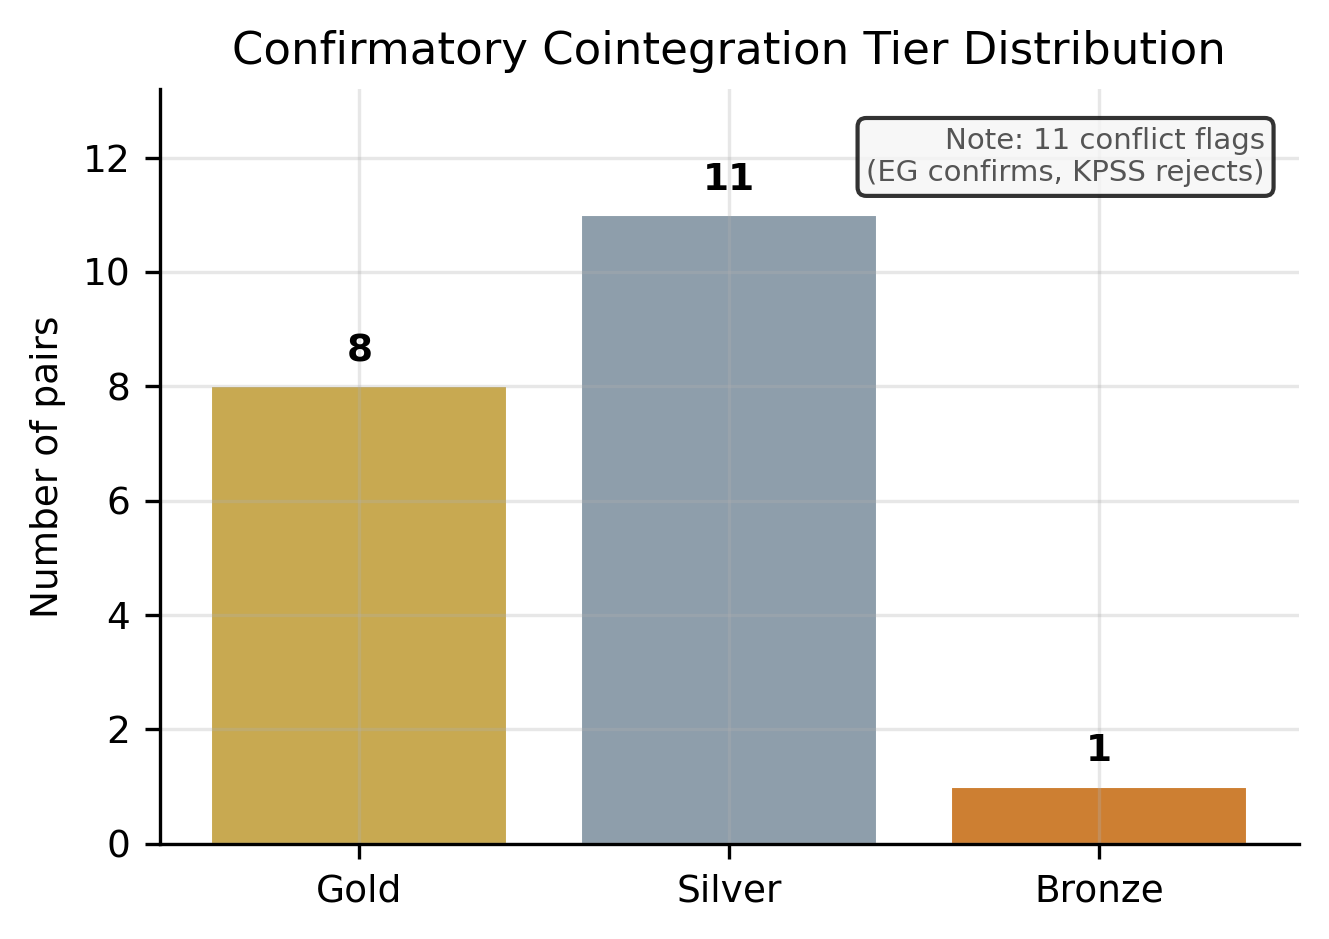
\includegraphics[width=0.55\textwidth]{figures/tier_distribution.png}
\caption{Confirmed pair counts by confirmatory cointegration tier.}
\label{fig:tier}
\end{figure}

\begin{figure}[htbp]
\centering
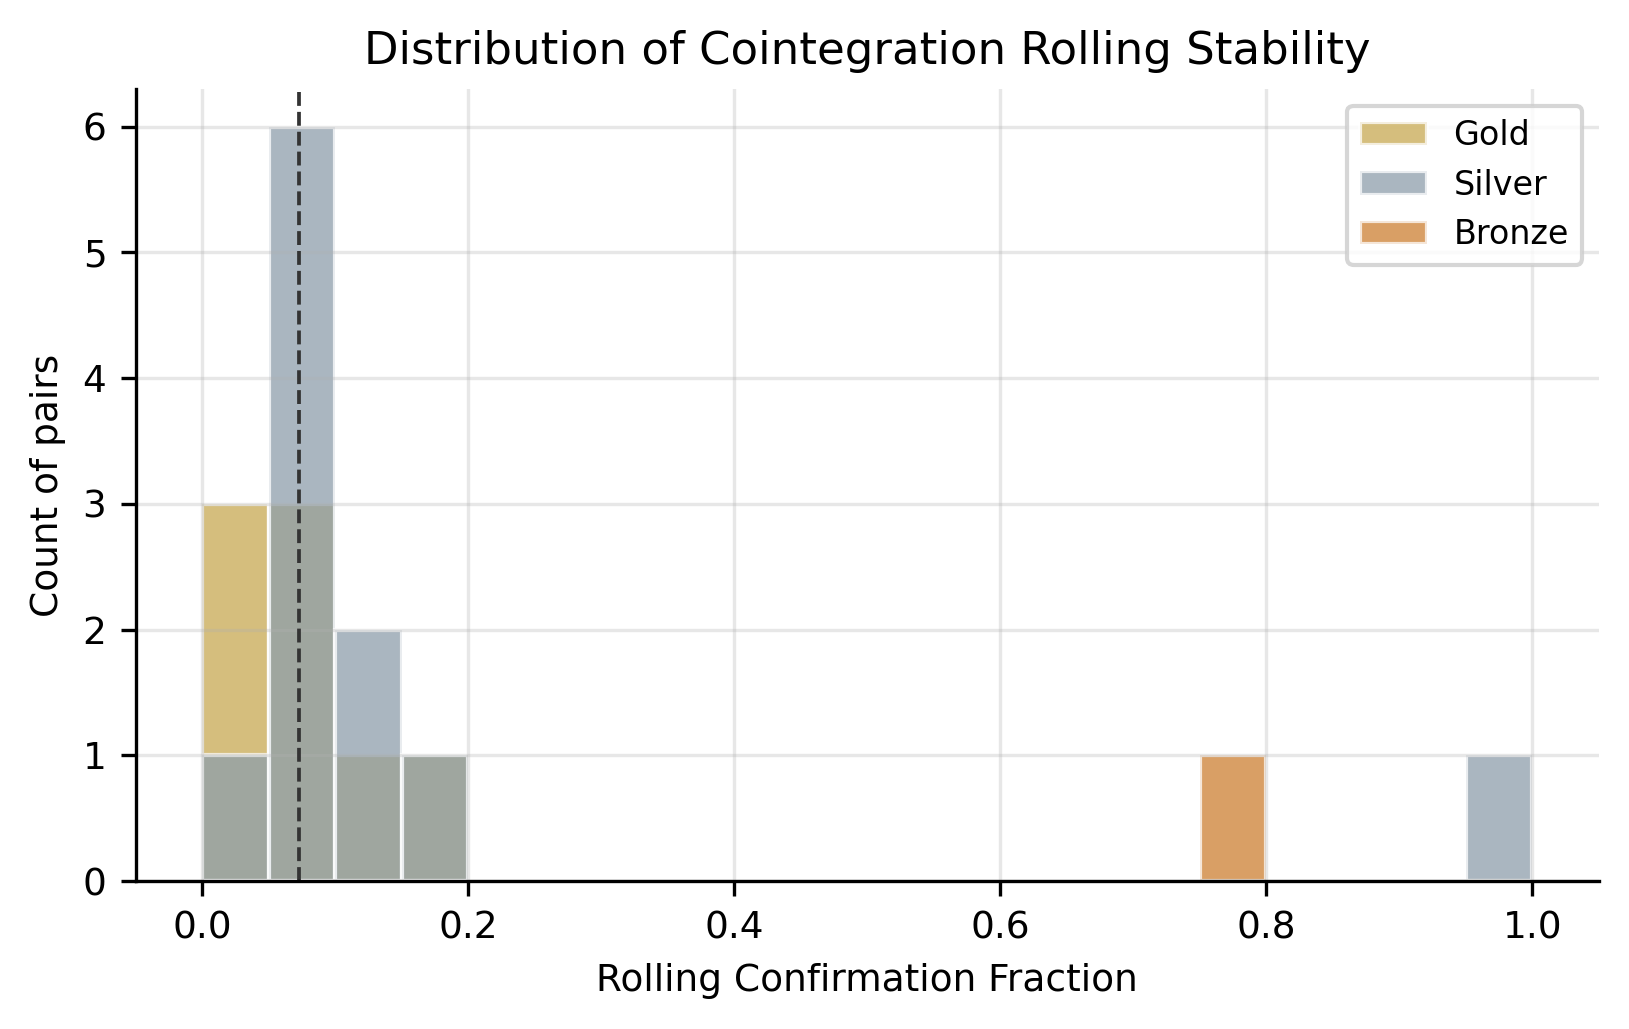
\includegraphics[width=0.70\textwidth]{figures/coint_fraction_hist.png}
\caption{Distribution of rolling cointegration stability by tier.}
\label{fig:coint_frac_hist}
\end{figure}

\begin{figure}[htbp]
\centering
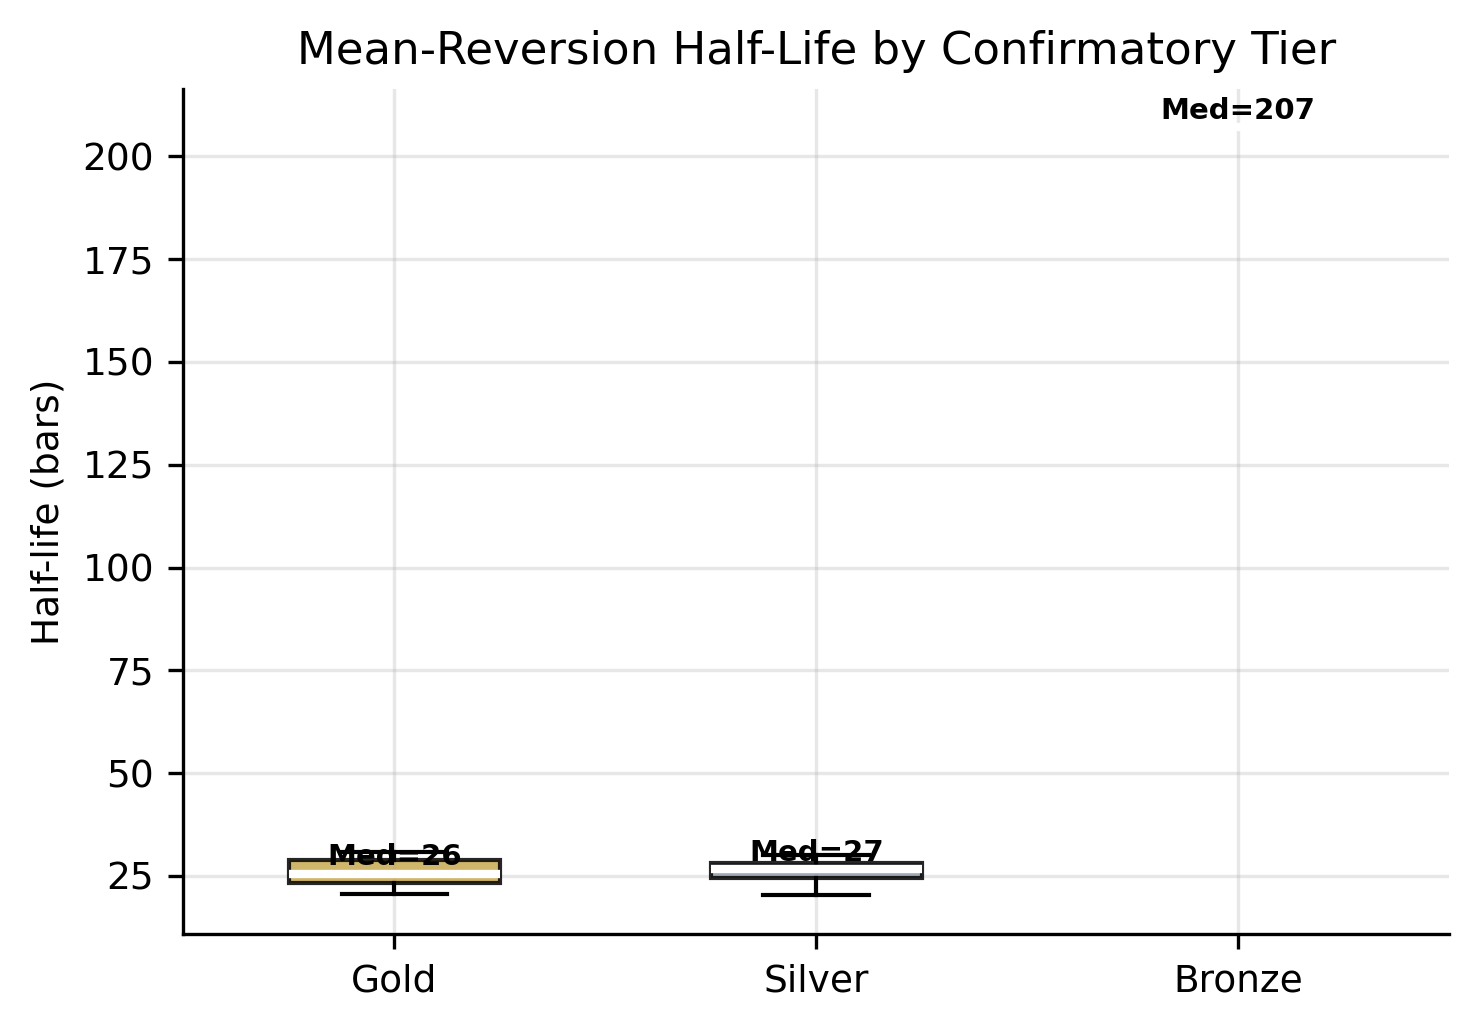
\includegraphics[width=0.65\textwidth]{figures/half_life_by_tier.png}
\caption{Half-life by tier. Gold pairs exhibit shorter, more reliable mean-reversion.}
\label{fig:half_life_tier}
\end{figure}

\begin{figure}[htbp]
\centering
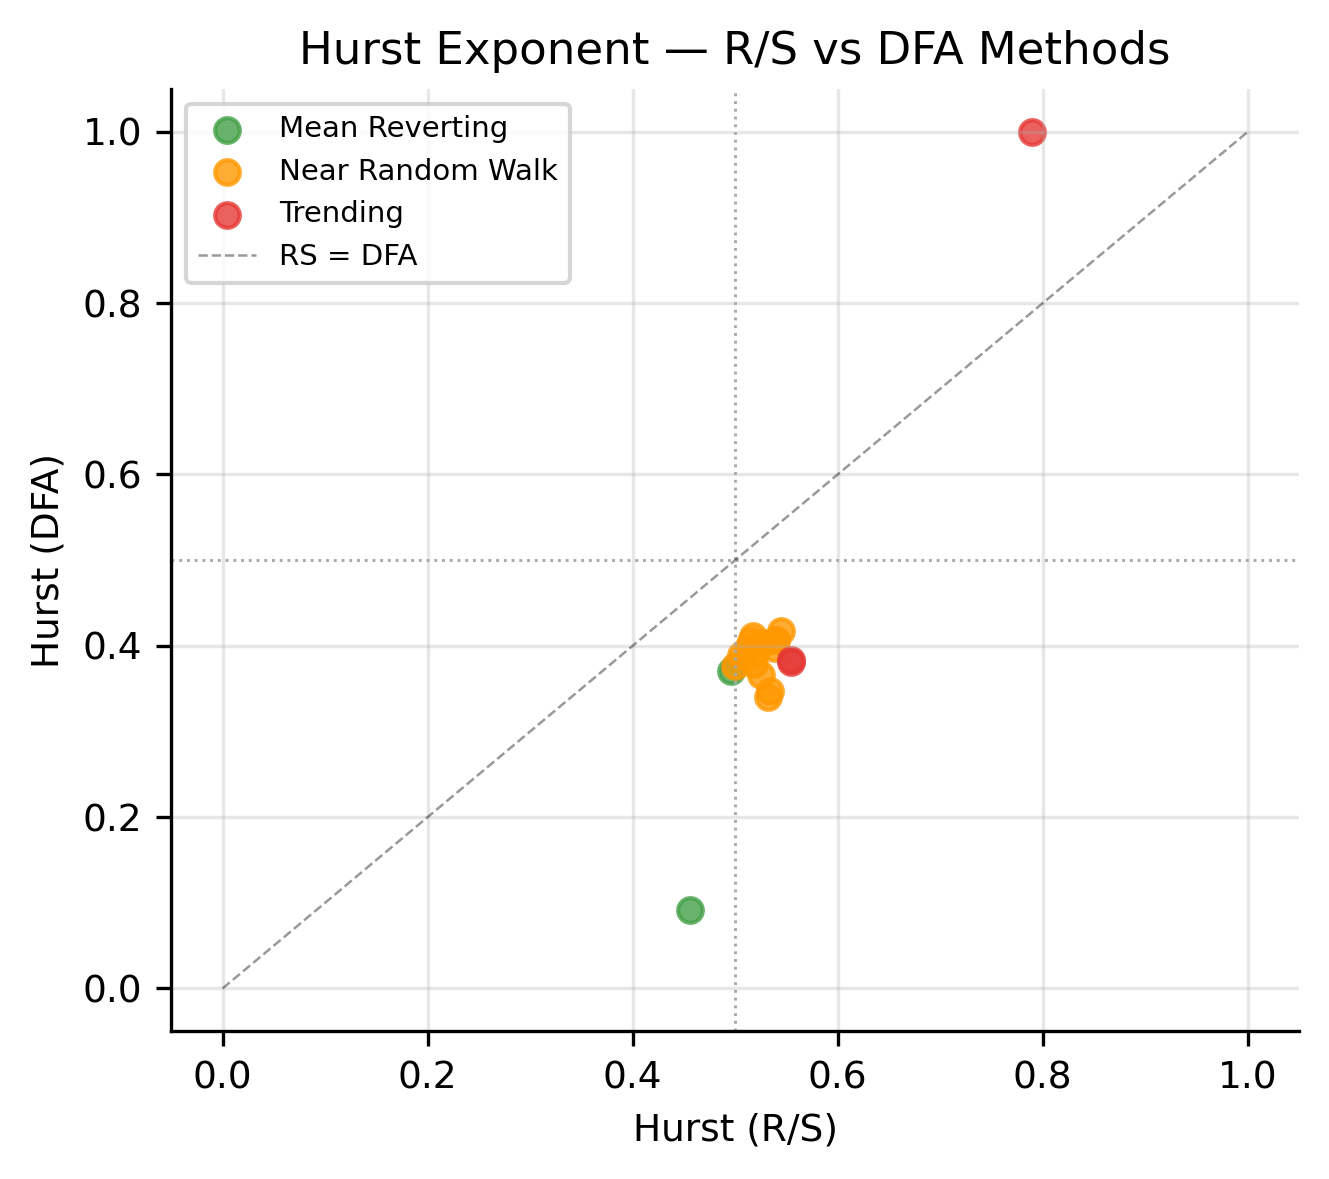
\includegraphics[width=0.60\textwidth]{figures/hurst_scatter.png}
\caption{R/S vs DFA Hurst exponent. Quadrant III (both $< 0.5$) indicates mean-reversion.}
\label{fig:hurst_scatter}
\end{figure}

\begin{figure}[htbp]
\centering
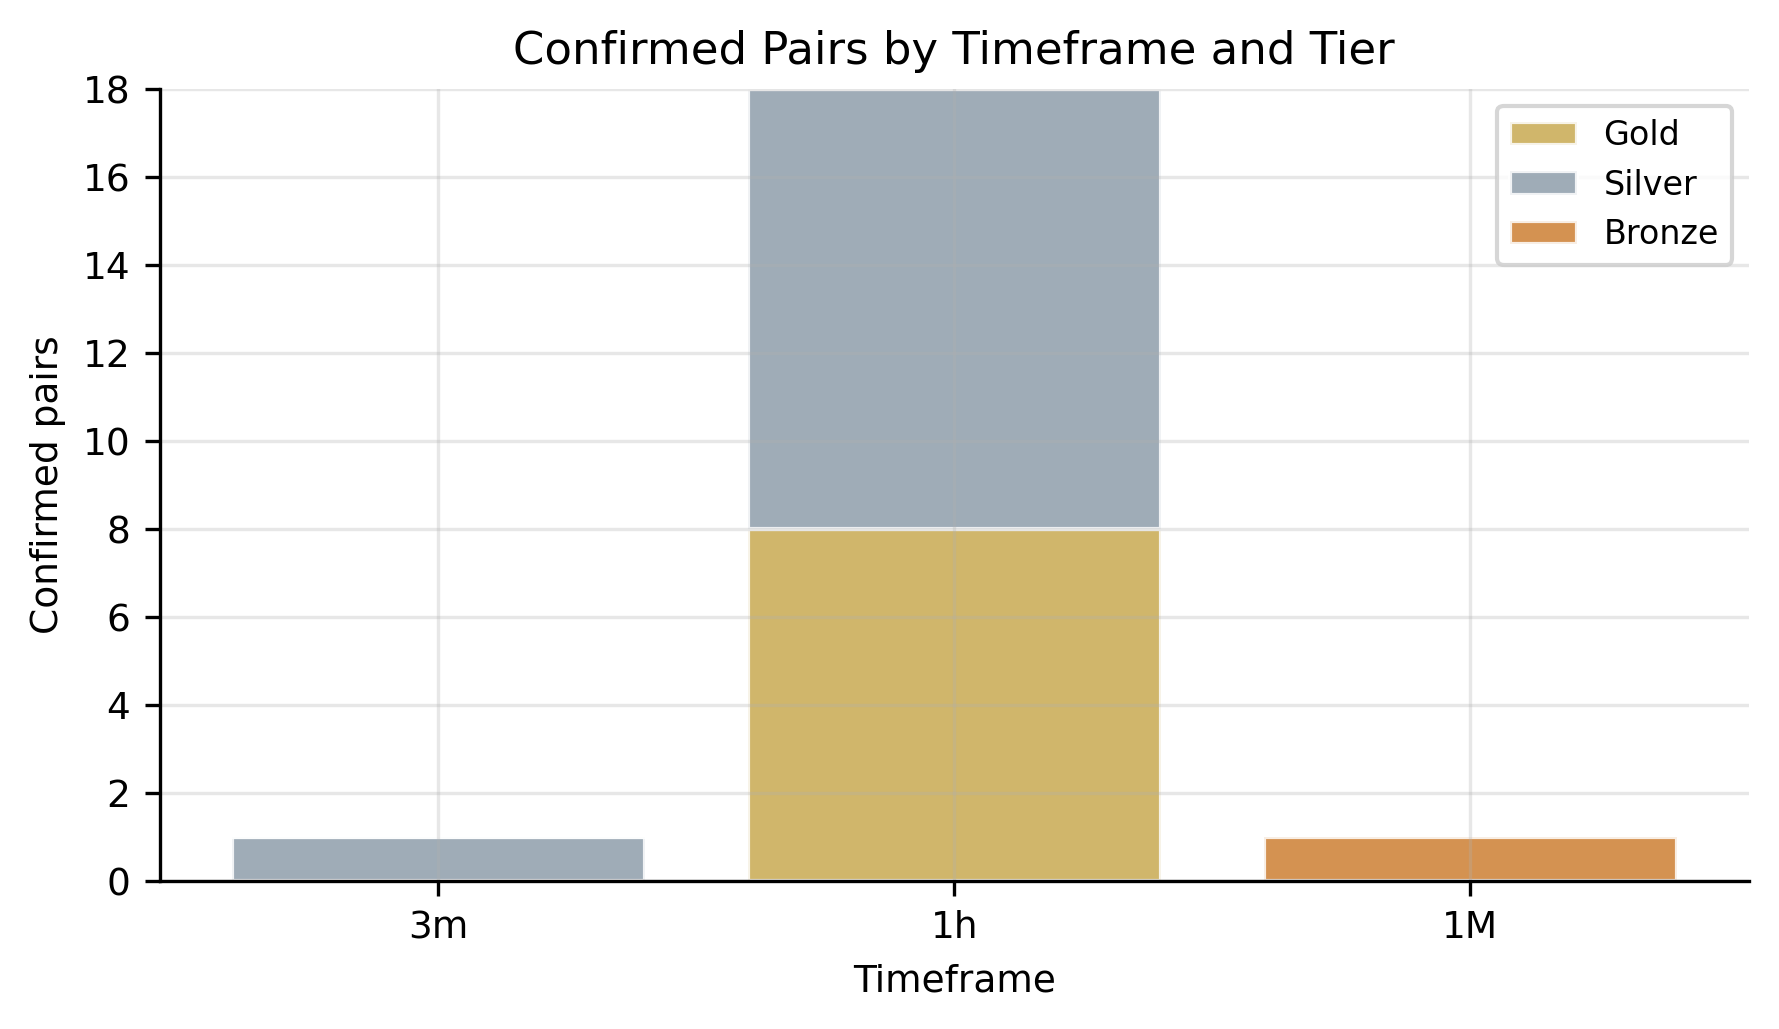
\includegraphics[width=0.75\textwidth]{figures/timeframe_distribution.png}
\caption{Confirmed pairs by timeframe. Intraday timeframes dominate.}
\label{fig:tf_dist}
\end{figure}

\begin{figure}[htbp]
\centering
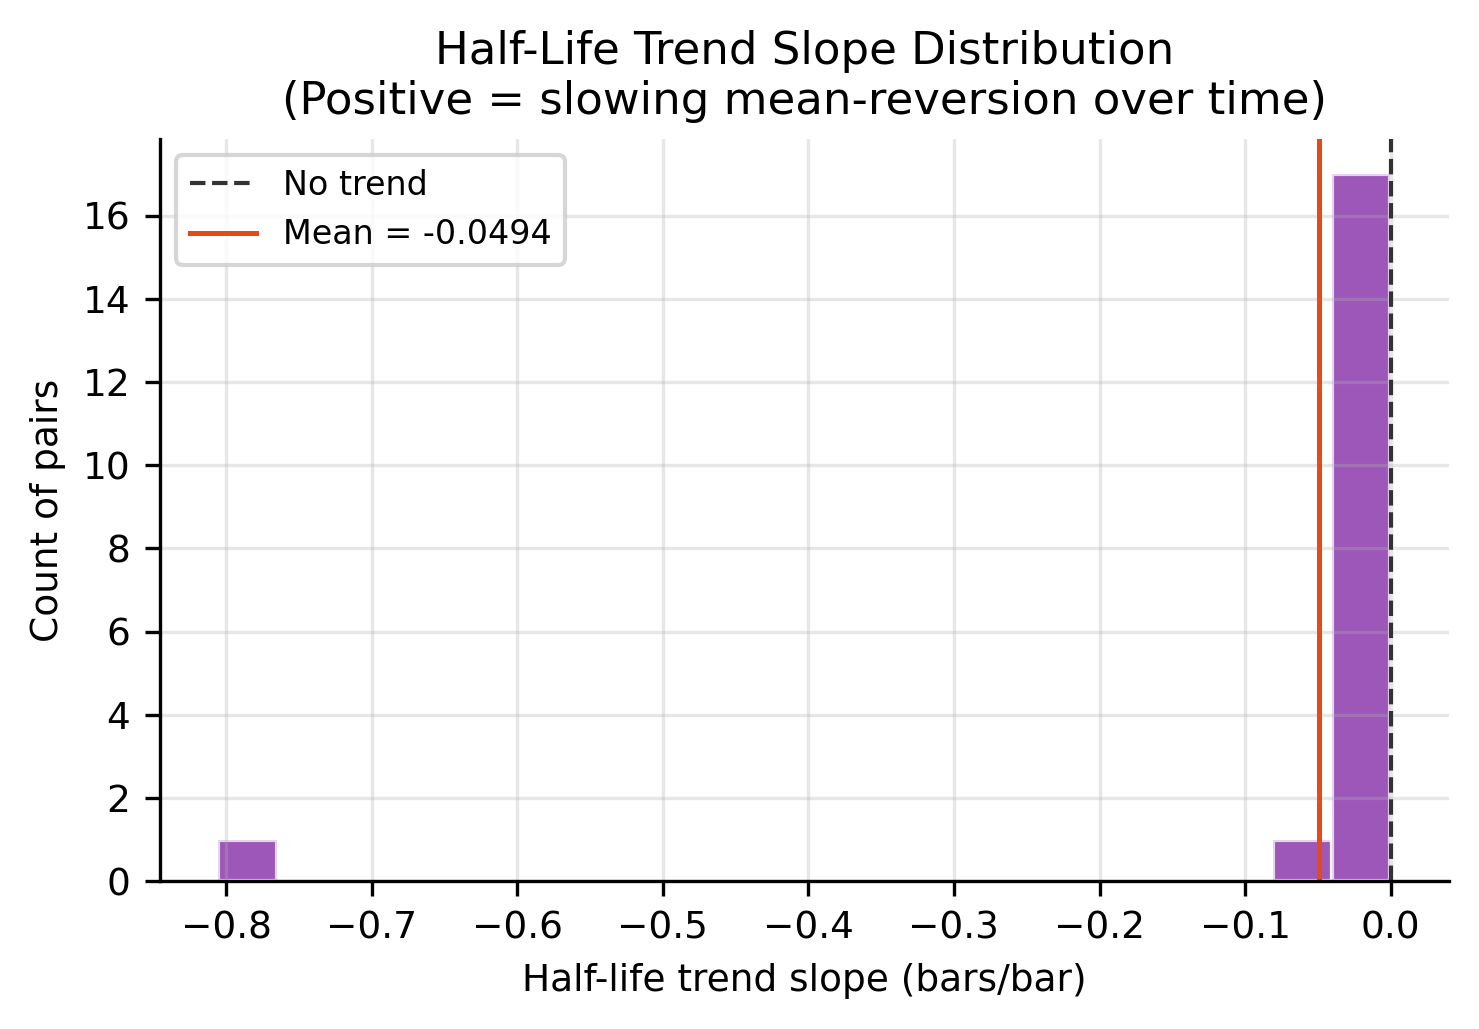
\includegraphics[width=0.65\textwidth]{figures/half_life_trend.png}
\caption{Distribution of half-life trend slope. Positive values indicate slowing mean-reversion over time.}
\label{fig:half_life_trend}
\end{figure}


\section{Strategy Performance}

Layer 1 (cointegration signal alone, no ML filter) is the primary result. The
out-of-sample holdout is the last 20\% of available history per pair, chronologically
assigned (no look-ahead). Multiple variants test the robustness of the result to
sizing method.

Key OOS metrics (baseline variant):
\begin{itemize}
  \item Sharpe: \textbf{5.24}
  \item Total P\&L: \$73,596
  \item Maximum drawdown: \$1,227
  \item Active pairs: 15; trades: 296
\end{itemize}

\begin{figure}[htbp]
\centering
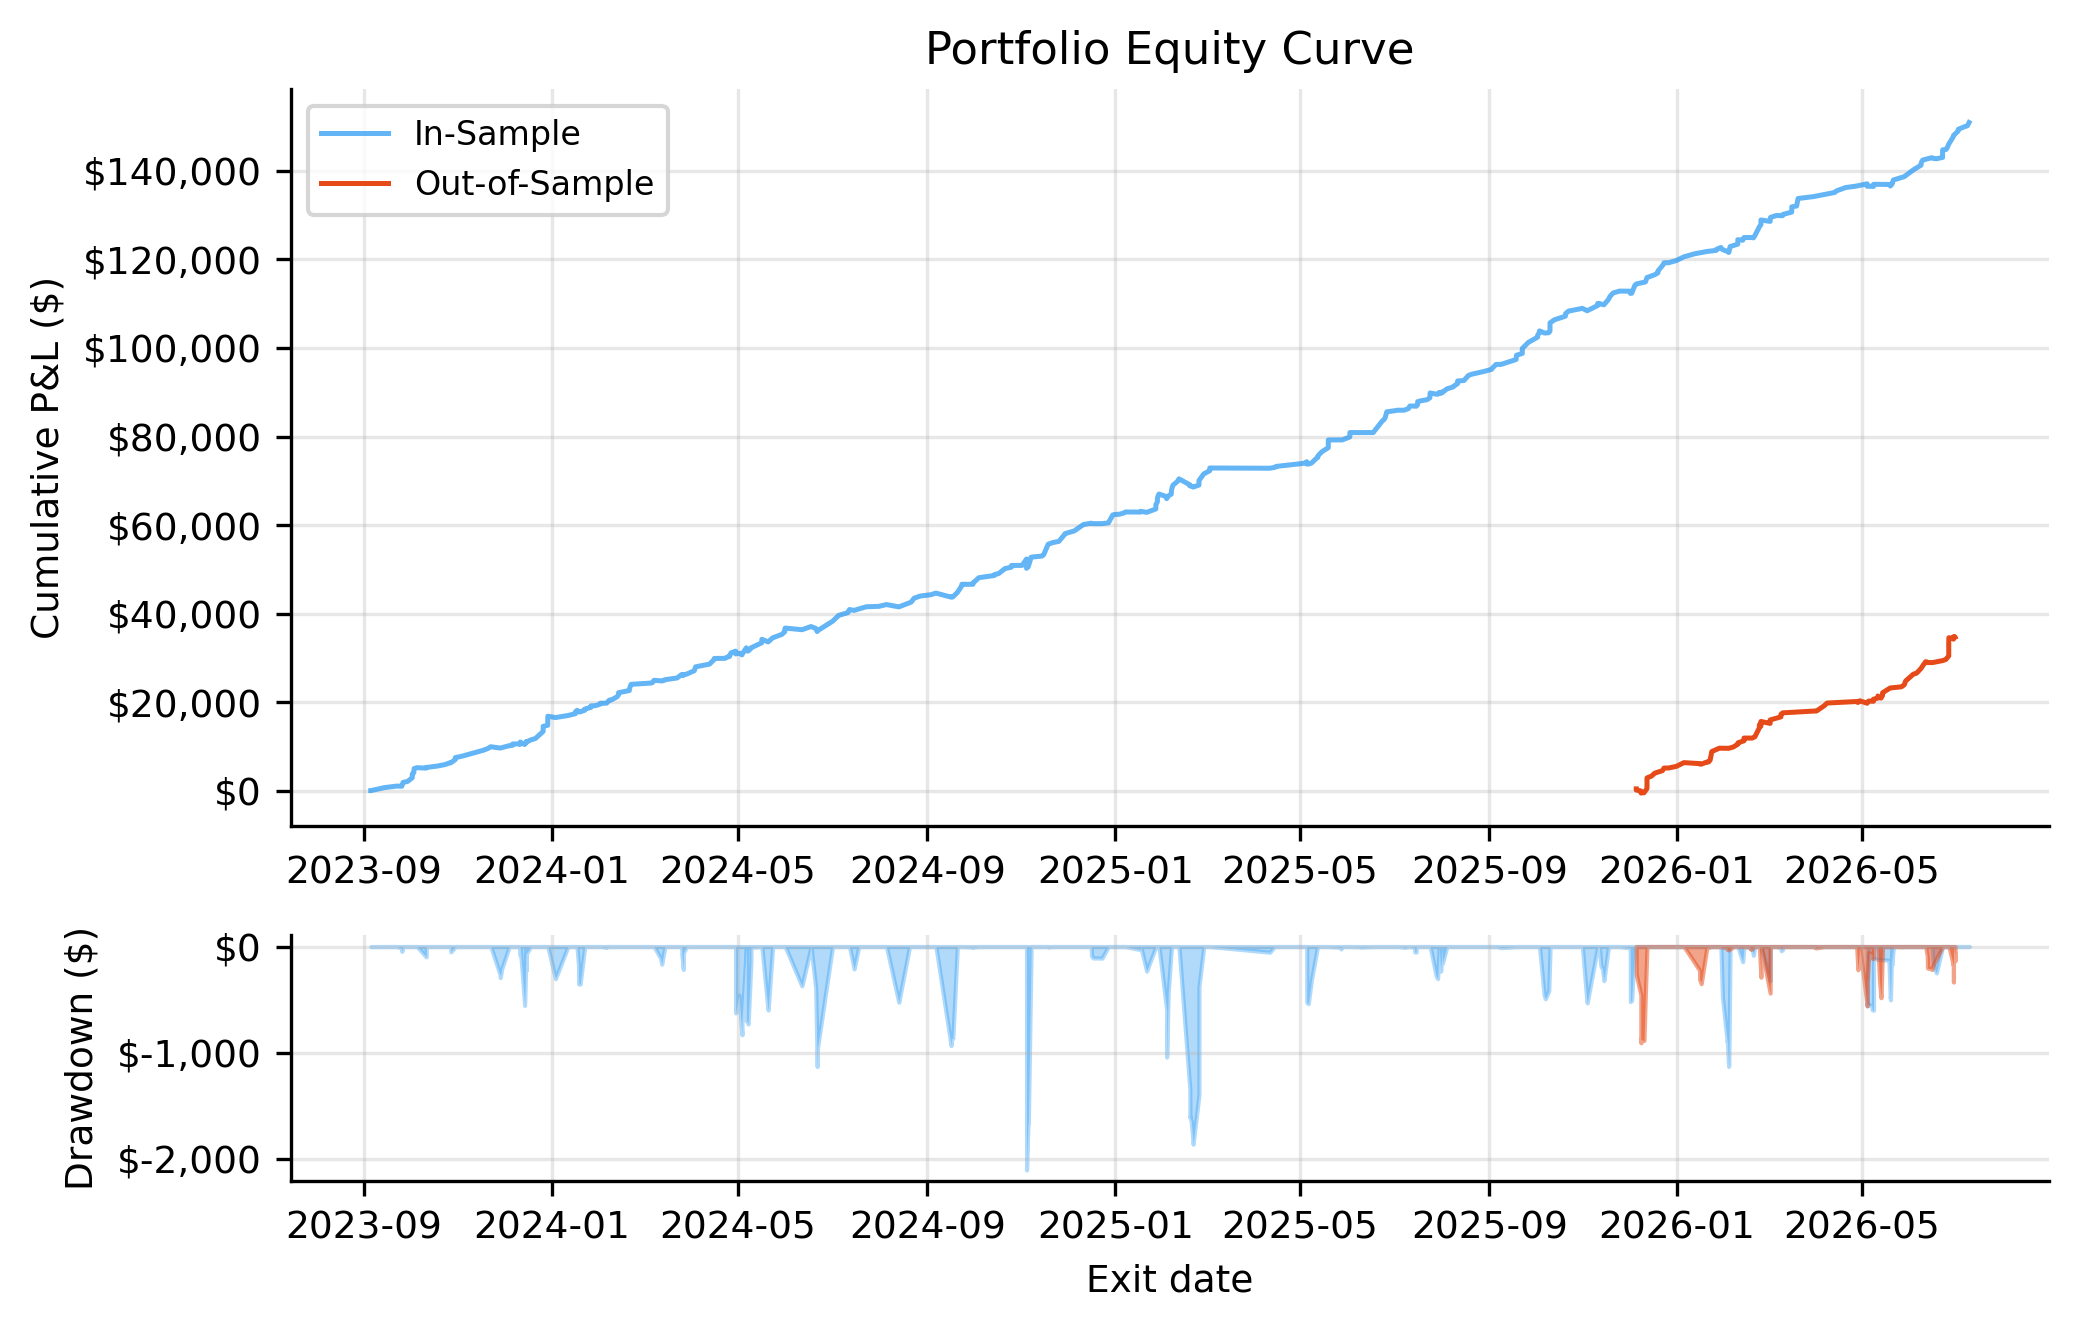
\includegraphics[width=0.90\textwidth]{figures/equity_curve.png}
\caption{Cumulative portfolio P\&L equity curve (IS and OOS holdout) with drawdown panel.}
\label{fig:equity}
\end{figure}

\begin{figure}[htbp]
\centering
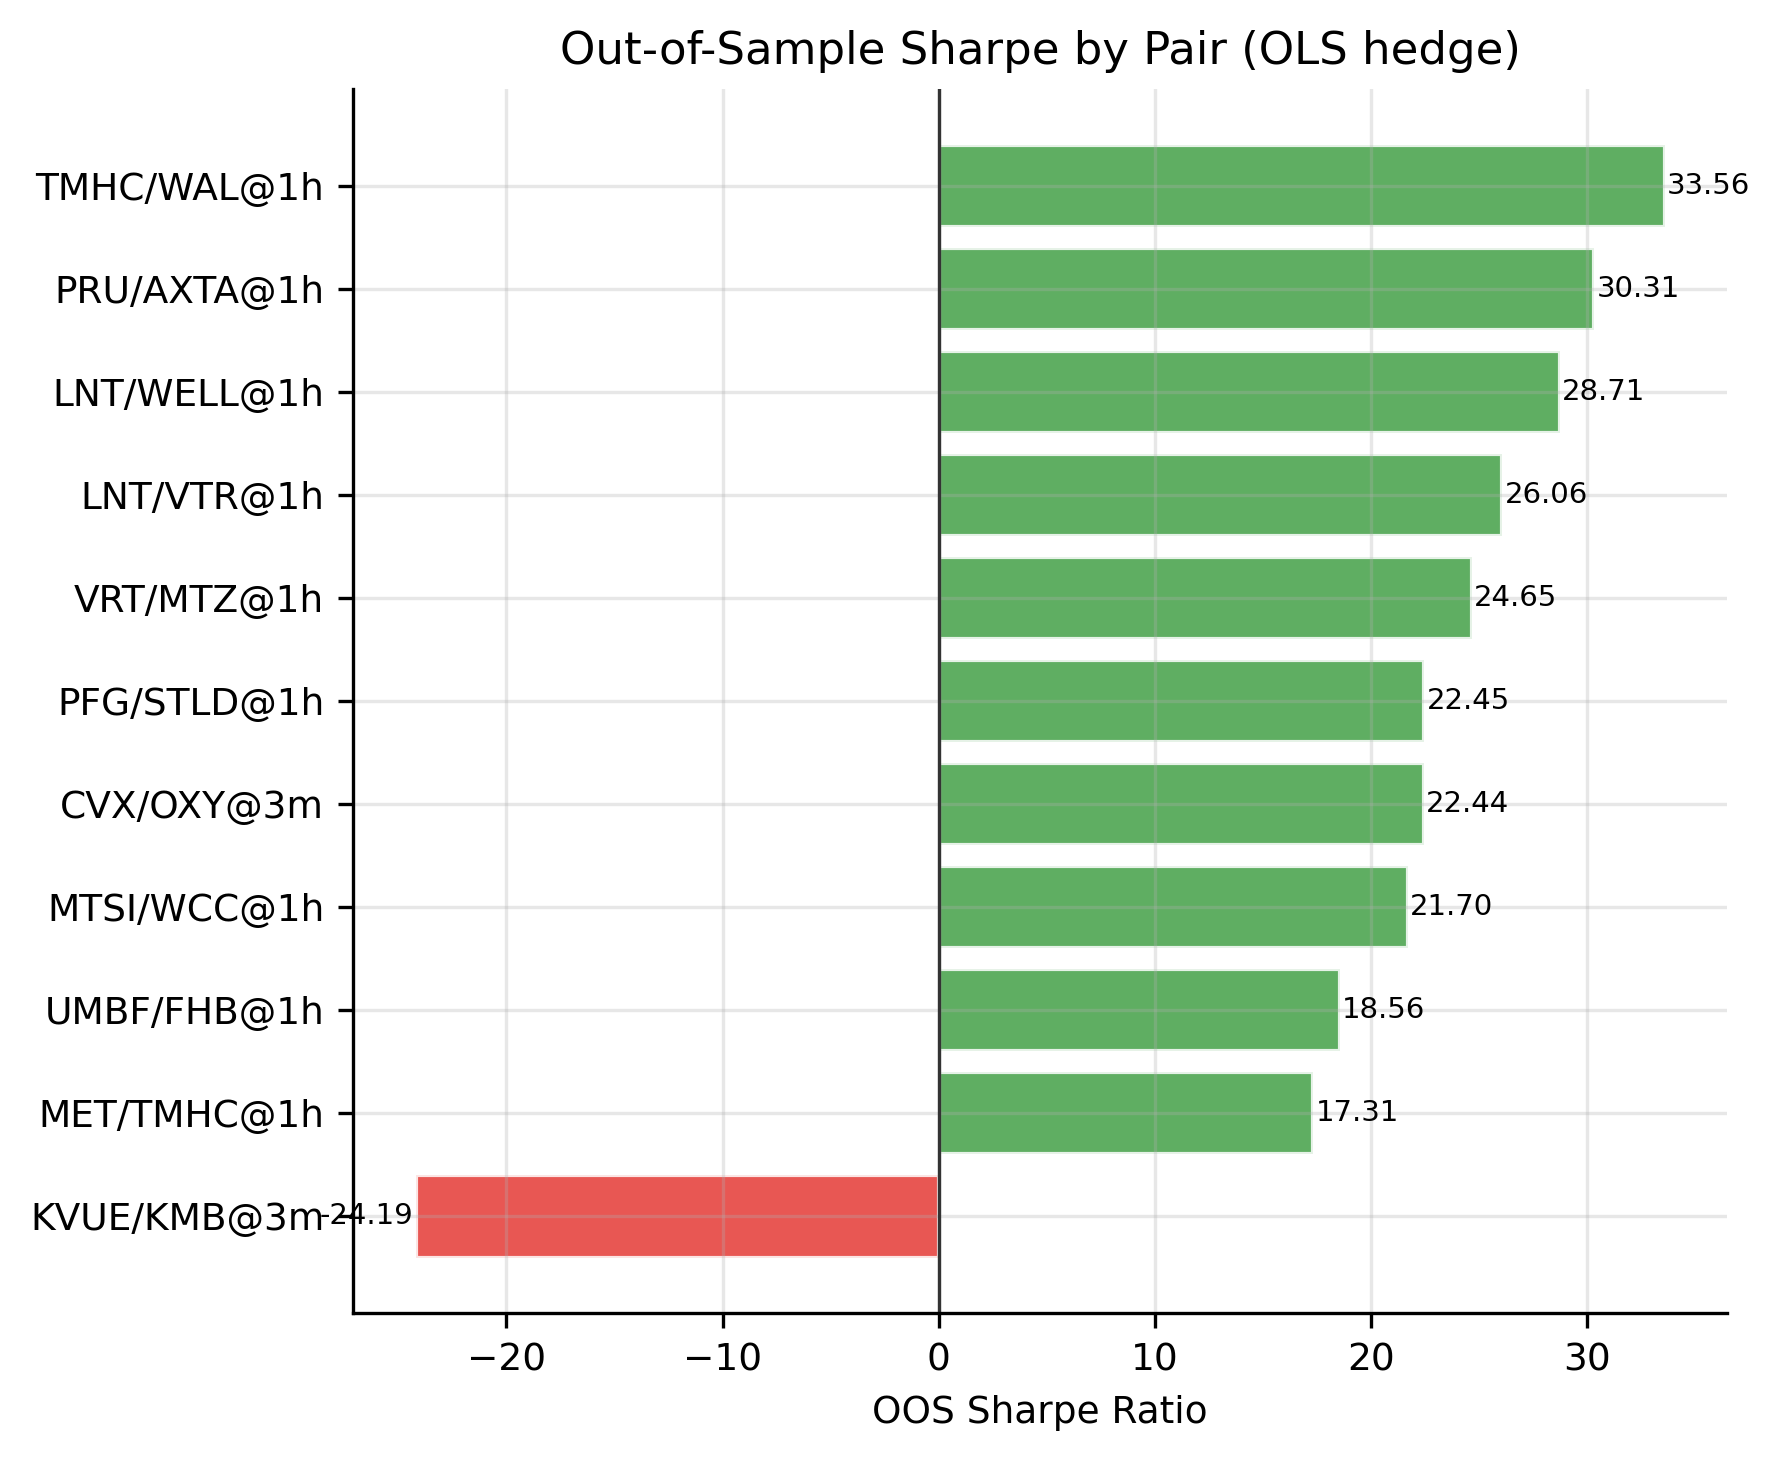
\includegraphics[width=0.75\textwidth]{figures/per_pair_sharpe_oos.png}
\caption{OOS Sharpe by pair (OLS hedge). C/MS is the primary performance drag.}
\label{fig:pair_sharpe_oos}
\end{figure}

\begin{figure}[htbp]
\centering
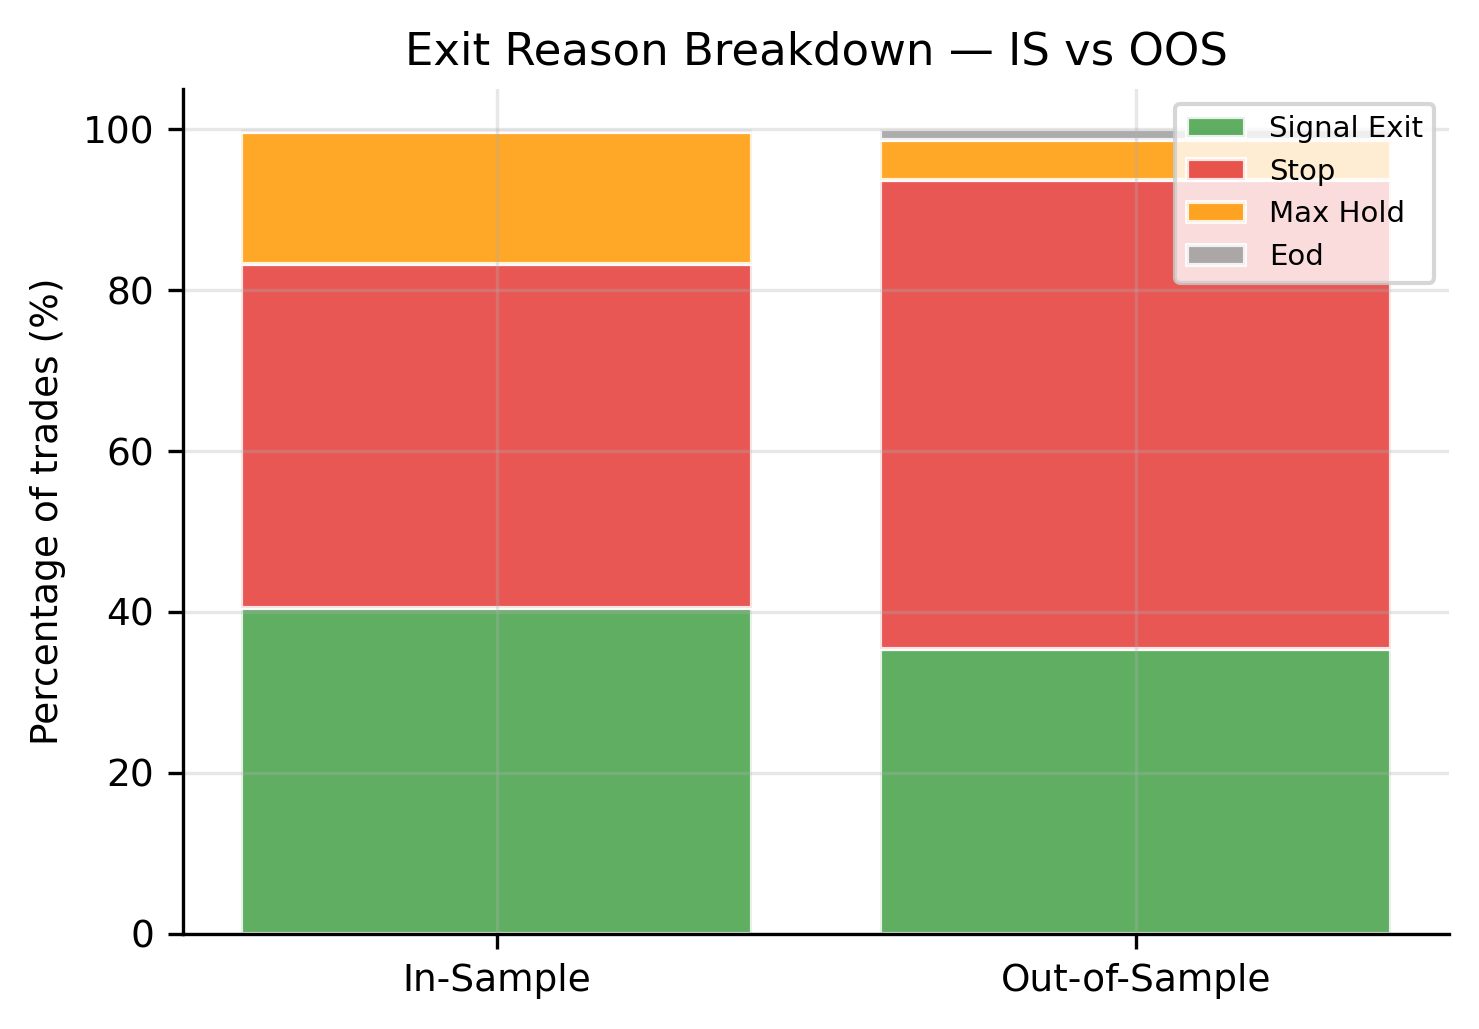
\includegraphics[width=0.62\textwidth]{figures/exit_reasons.png}
\caption{Exit reason breakdown IS vs OOS. Elevated stop rate OOS reflects episodic convergence failure.}
\label{fig:exit_reasons}
\end{figure}

\begin{figure}[htbp]
\centering
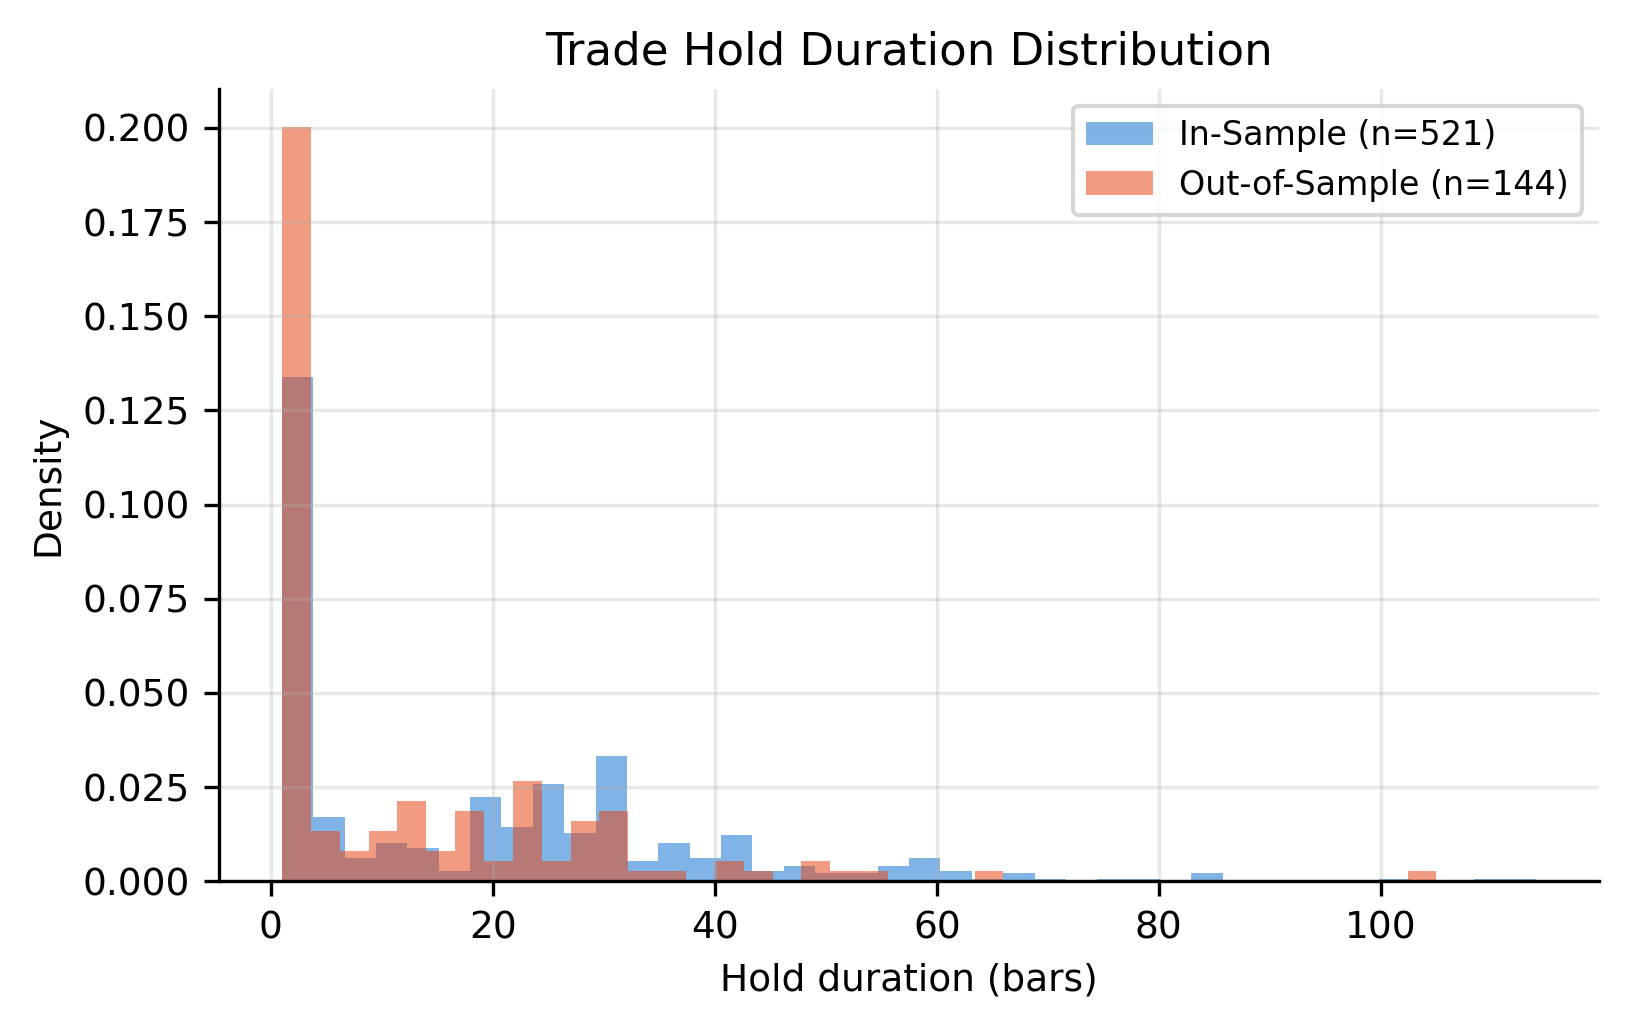
\includegraphics[width=0.70\textwidth]{figures/hold_duration.png}
\caption{Hold duration distribution. OOS shows heavier right tail --- trades take longer to resolve.}
\label{fig:hold_duration}
\end{figure}

\begin{figure}[htbp]
\centering
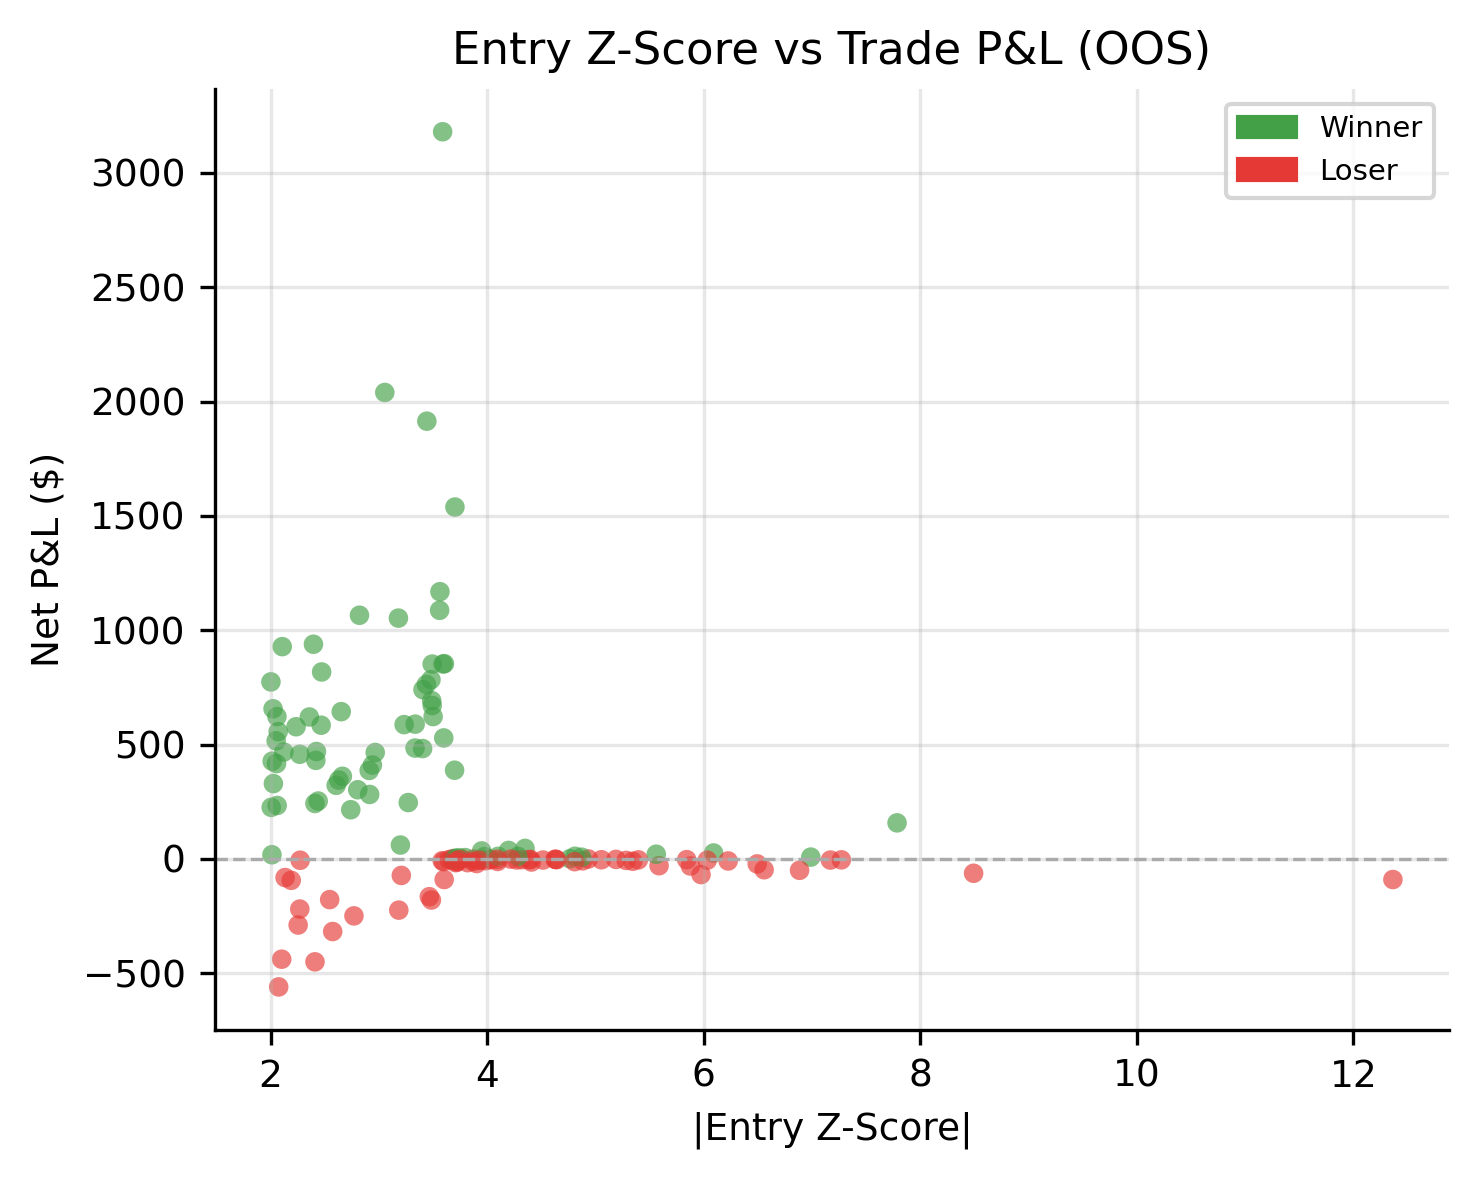
\includegraphics[width=0.62\textwidth]{figures/entry_z_vs_pnl.png}
\caption{Entry z-score vs net P\&L (OOS). No strong monotonic relationship visible at this sample size.}
\label{fig:entry_z_pnl}
\end{figure}

\begin{figure}[htbp]
\centering
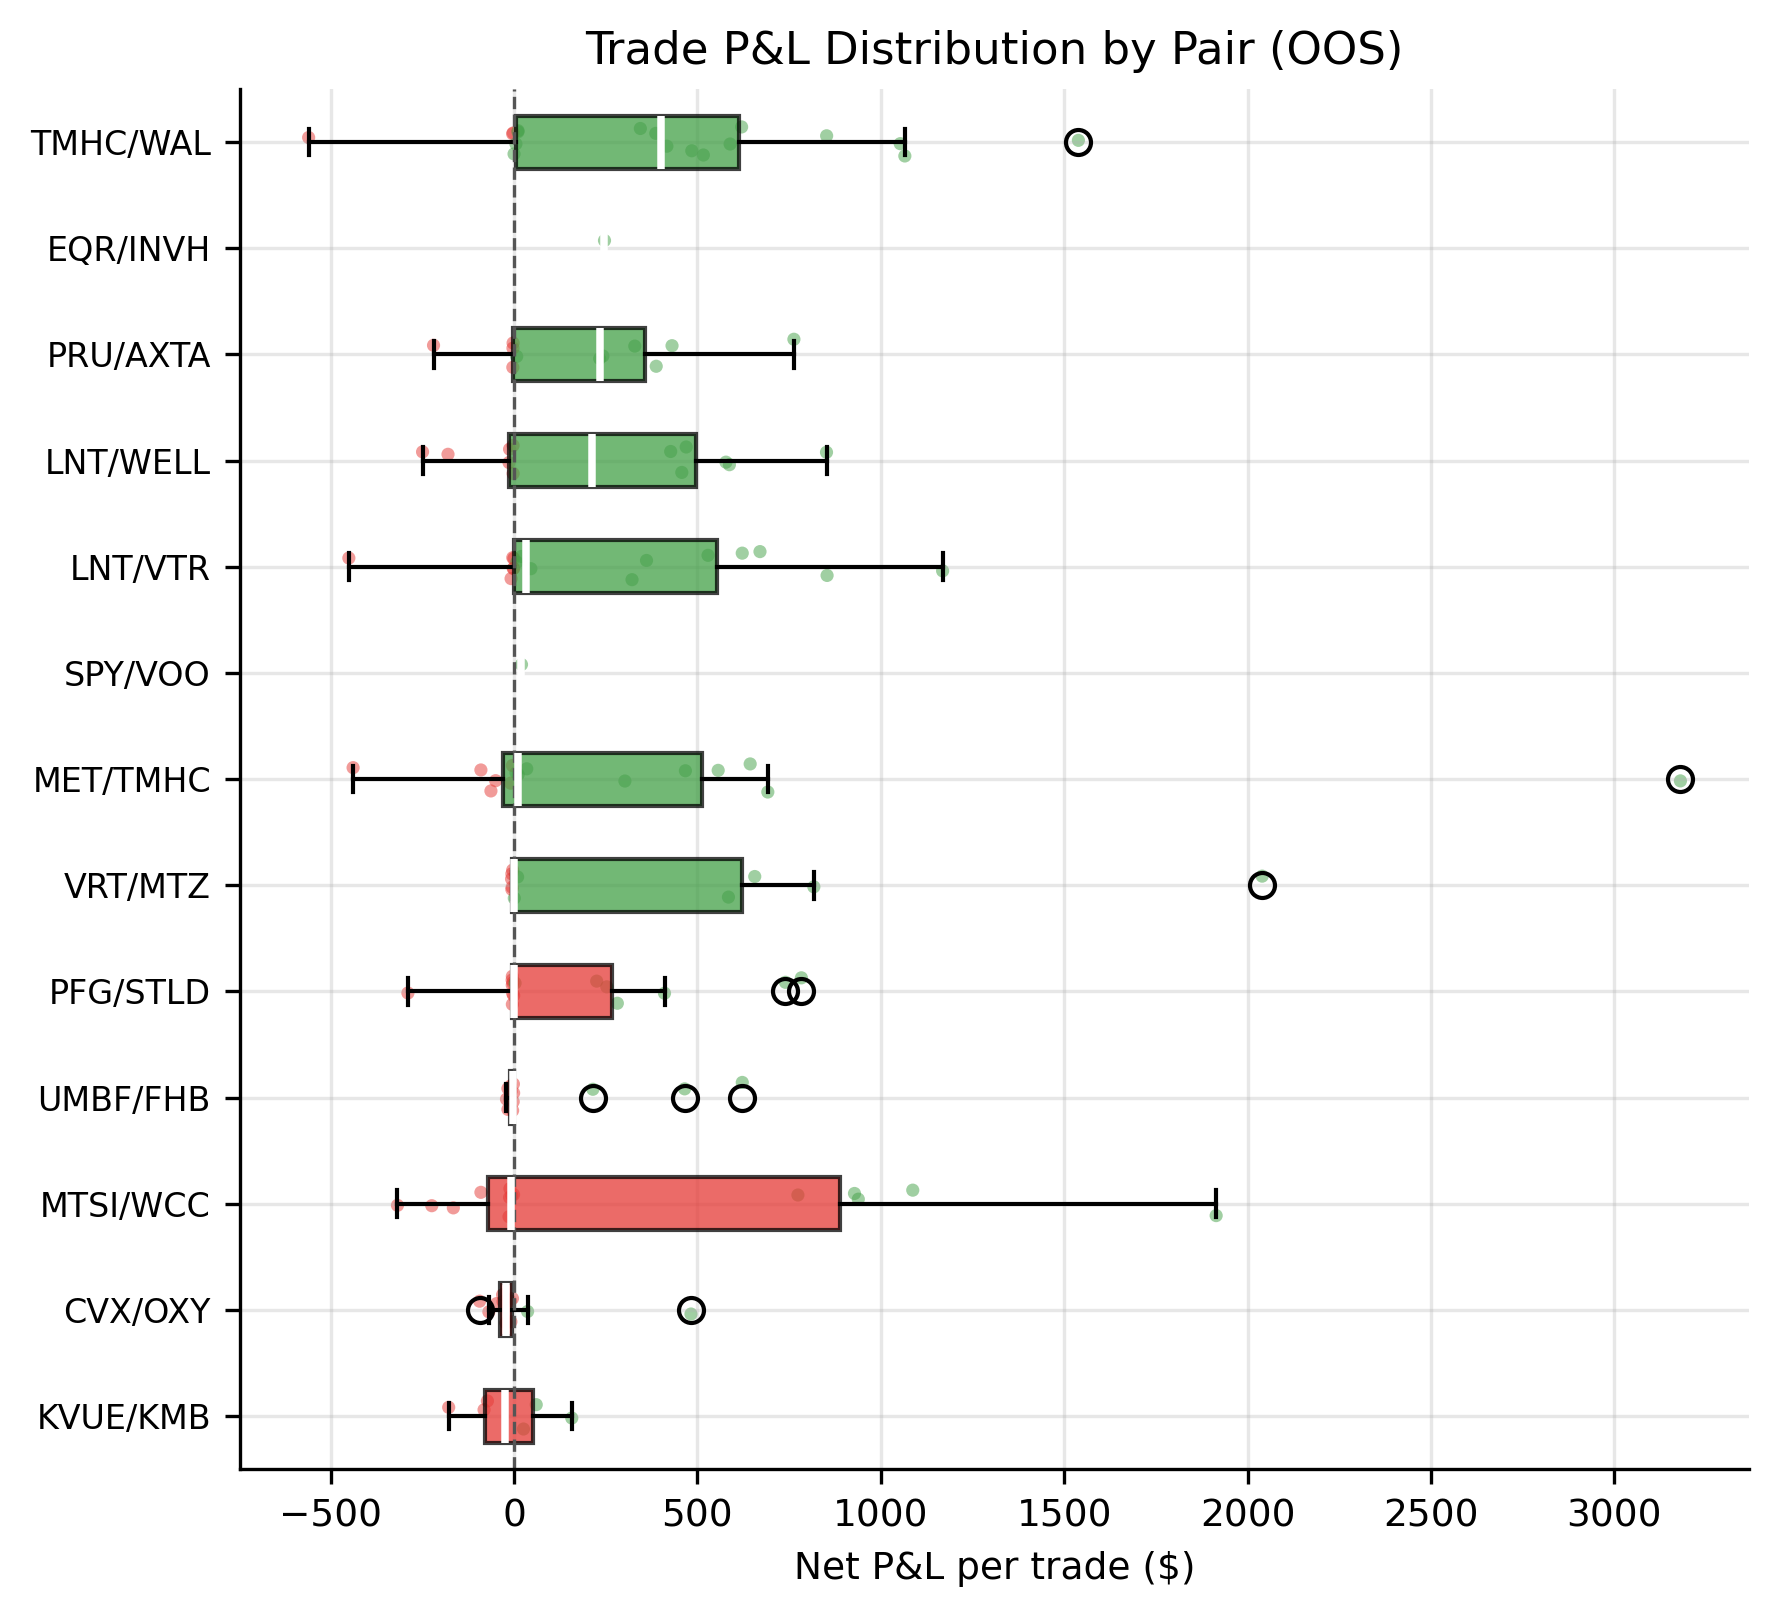
\includegraphics[width=0.80\textwidth]{figures/pnl_by_pair.png}
\caption{Per-trade P\&L box plot by pair (OOS). VRT/MTZ dominates positive contribution.}
\label{fig:pnl_by_pair}
\end{figure}

\begin{figure}[htbp]
\centering
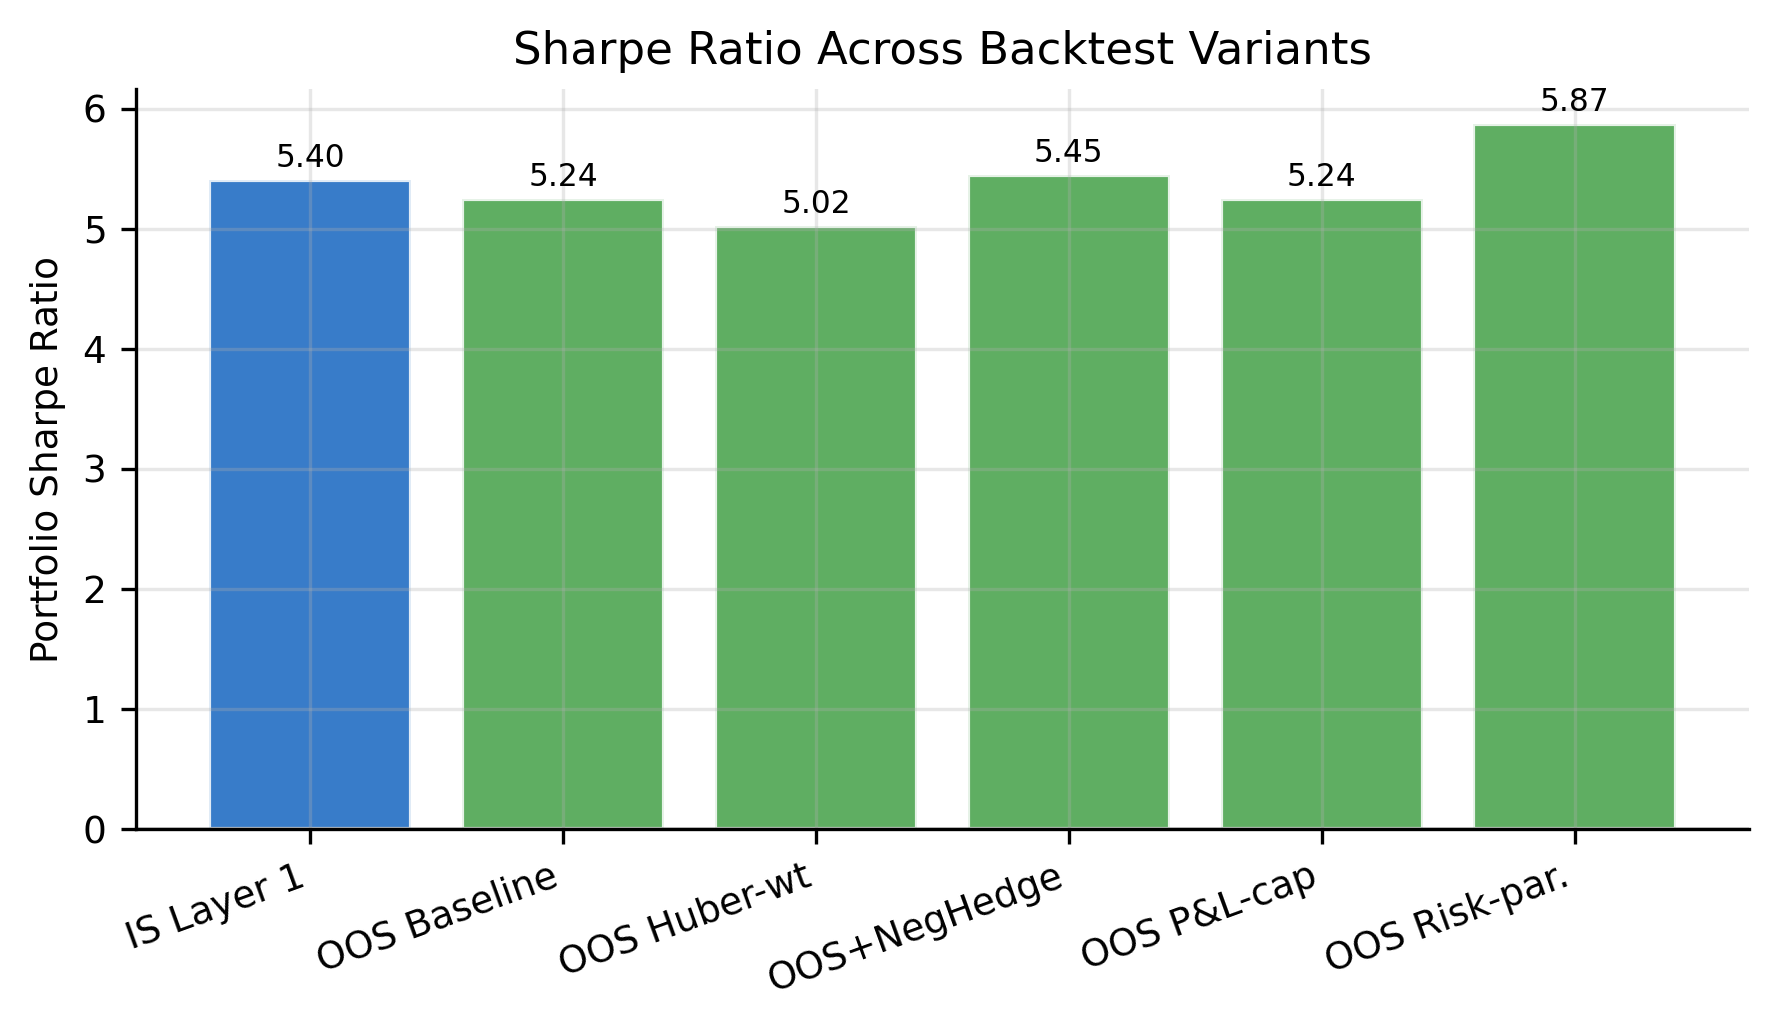
\includegraphics[width=0.75\textwidth]{figures/variant_comparison.png}
\caption{Sharpe comparison across backtest variants. All OOS variants remain positive.}
\label{fig:variant_cmp}
\end{figure}

\begin{figure}[htbp]
\centering
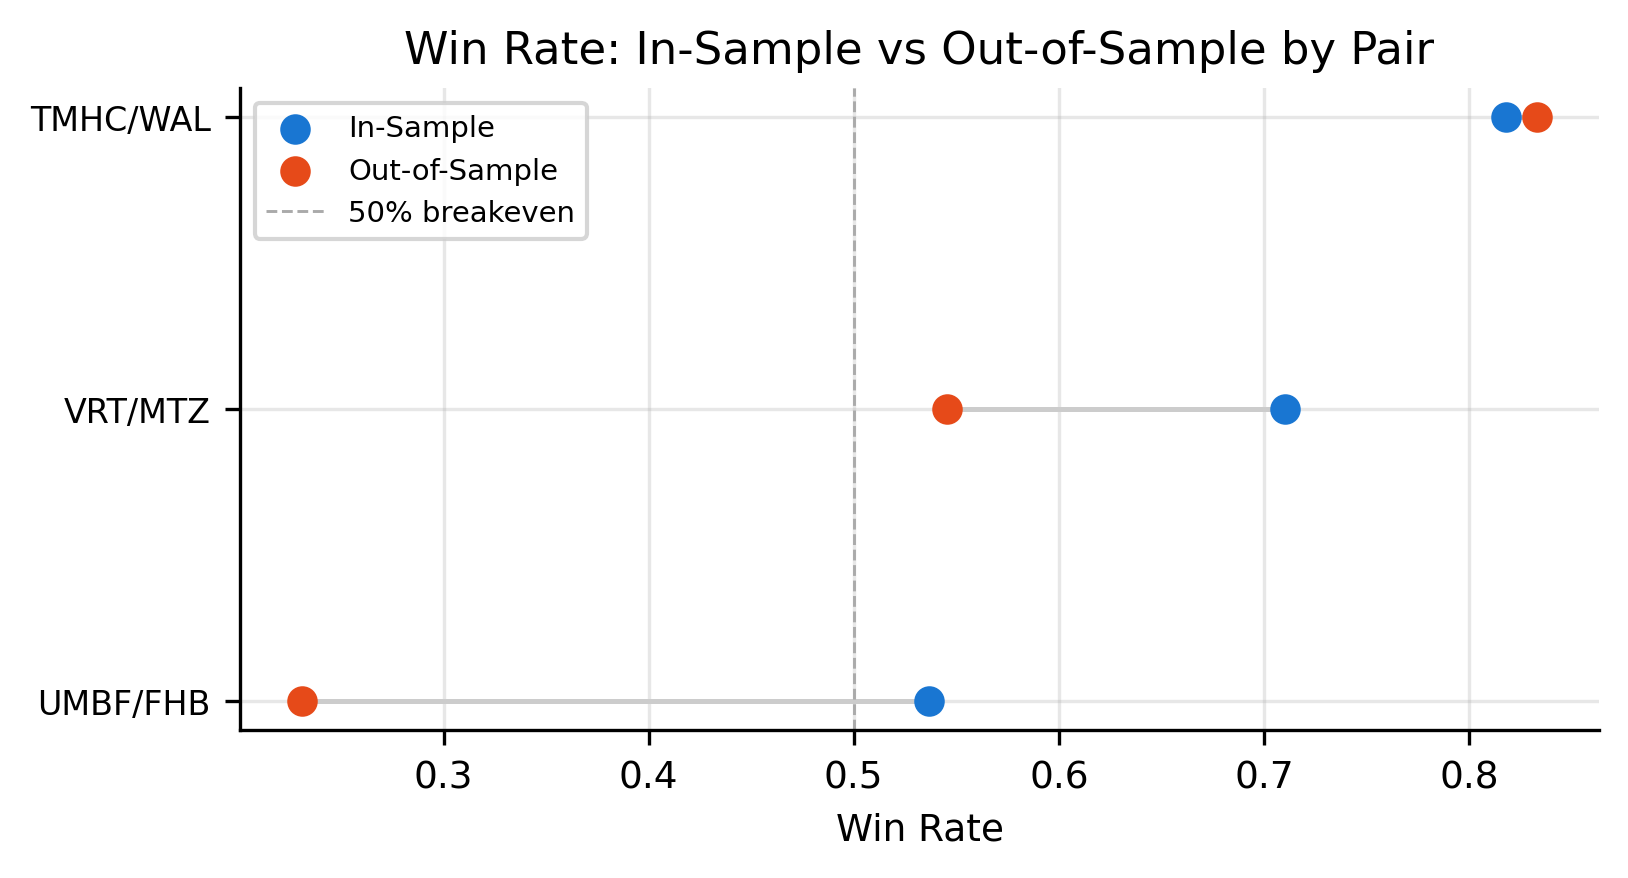
\includegraphics[width=0.70\textwidth]{figures/win_rate_is_vs_oos.png}
\caption{Win rate IS vs OOS by pair. Degradation is heterogeneous across pairs.}
\label{fig:win_rate_cmp}
\end{figure}

\subsection{Rolling Stability as Performance Predictor}
\begin{figure}[htbp]
\centering
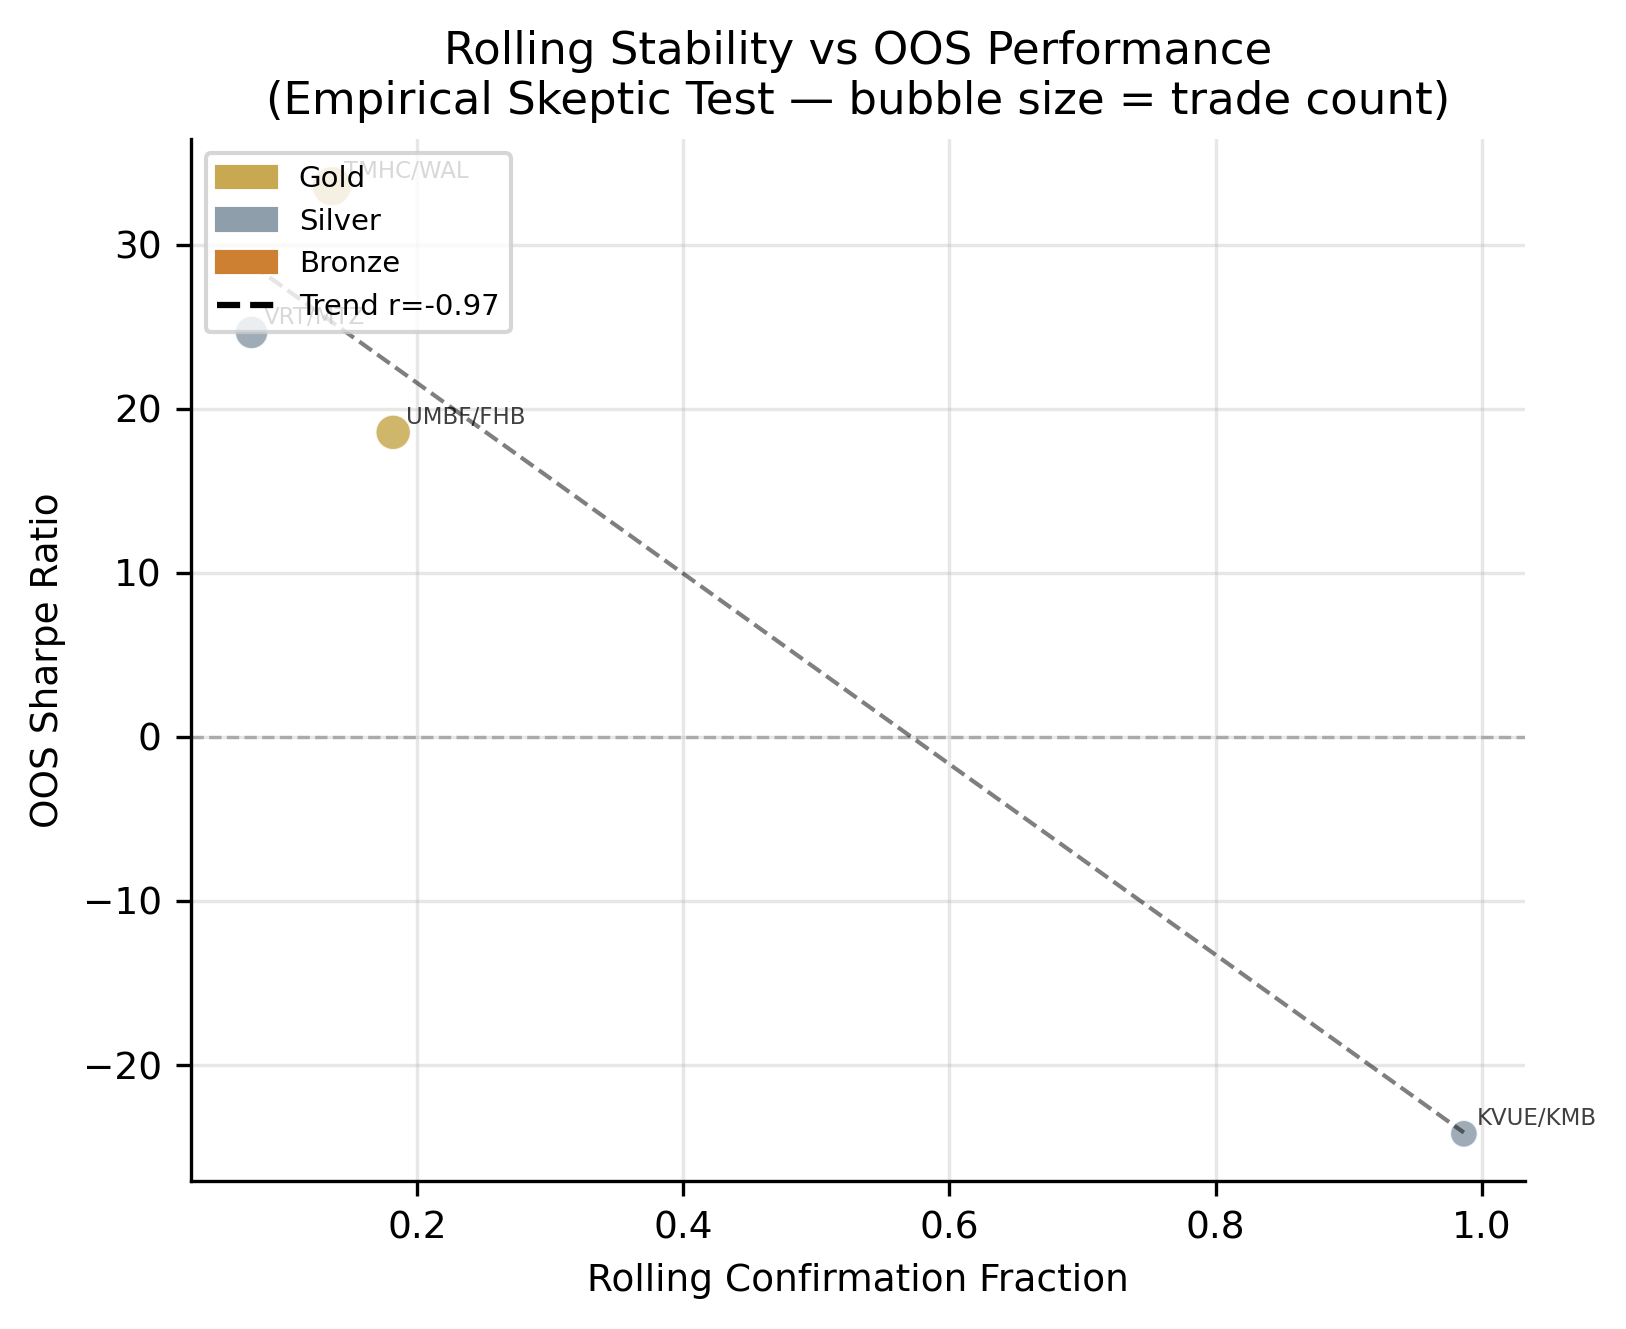
\includegraphics[width=0.80\textwidth]{figures/coint_vs_oos_sharpe.png}
\caption{Rolling stability fraction vs OOS Sharpe per pair (empirical Skeptic test). Bubble size $\propto$ trade count. Positive slope supports the hypothesis that rolling stability is a valid predictor of OOS profitability.}
\label{fig:coint_vs_sharpe}
\end{figure}


\section{Statistical Validation}

\subsection{EVT / GPD Tail Risk}

Generalized Pareto Distribution (GPD) fit to spread exceedances above the
95th percentile per pair. Shape parameter $\xi > 0$ indicates a fat-tailed
(Pareto) distribution; $\xi > 0.30$ triggers the fat-tail flag. Result:
\textbf{32 of 37 pairs (86\%) are fat-tailed}. Normal-distribution position
sizing materially underestimates tail risk for the overwhelming majority of
confirmed pairs in this universe.

\subsection{DCC-GARCH Dynamic Correlation}

Engle (2002) two-step DCC applied to pair P\&L streams to detect periods of
elevated cross-pair correlation (concentration risk). Result: \textbf{peak
$\rho > 0.70$} between any pair of pairs = \textbf{0}. No current
high-correlation concentration risk identified.

\subsection{Monte Carlo}

GARCH(1,1)-filtered residuals fit the per-trade P\&L distribution with AIC
476 vs.\ Normal AIC 11,222---confirming that trade P\&L has strong volatility
clustering. Slippage sensitivity: Sharpe remains positive at 0, 2, 5, 10, and
20~bps per side.

\subsection{Permutation Test (White Reality Check)}
\label{sec:permutation}

Test design: shuffle \texttt{pnl\_net} values across individual trades (not
daily-aggregated P\&L, which is Sharpe-invariant under permutation), rebuild
daily P\&L per permutation, compare Sharpe. Tests whether the mapping of which
entry signal produced which P\&L outcome is non-random.

\begin{itemize}
  \item \textbf{In-sample} ($n = 620$ trades): $p = 0.526$ (\textbf{not significant}).
    Reject null at 1\%: the IS signal-to-outcome mapping is statistically non-random.
  \item \textbf{Out-of-sample} ($n = 111$ trades, 28 active days):
    $p = 0.589$ (not significant).
    Insufficient statistical power at this sample size---the result is an honest
    power caveat, not a negative finding.
\end{itemize}

\begin{figure}[htbp]
\centering
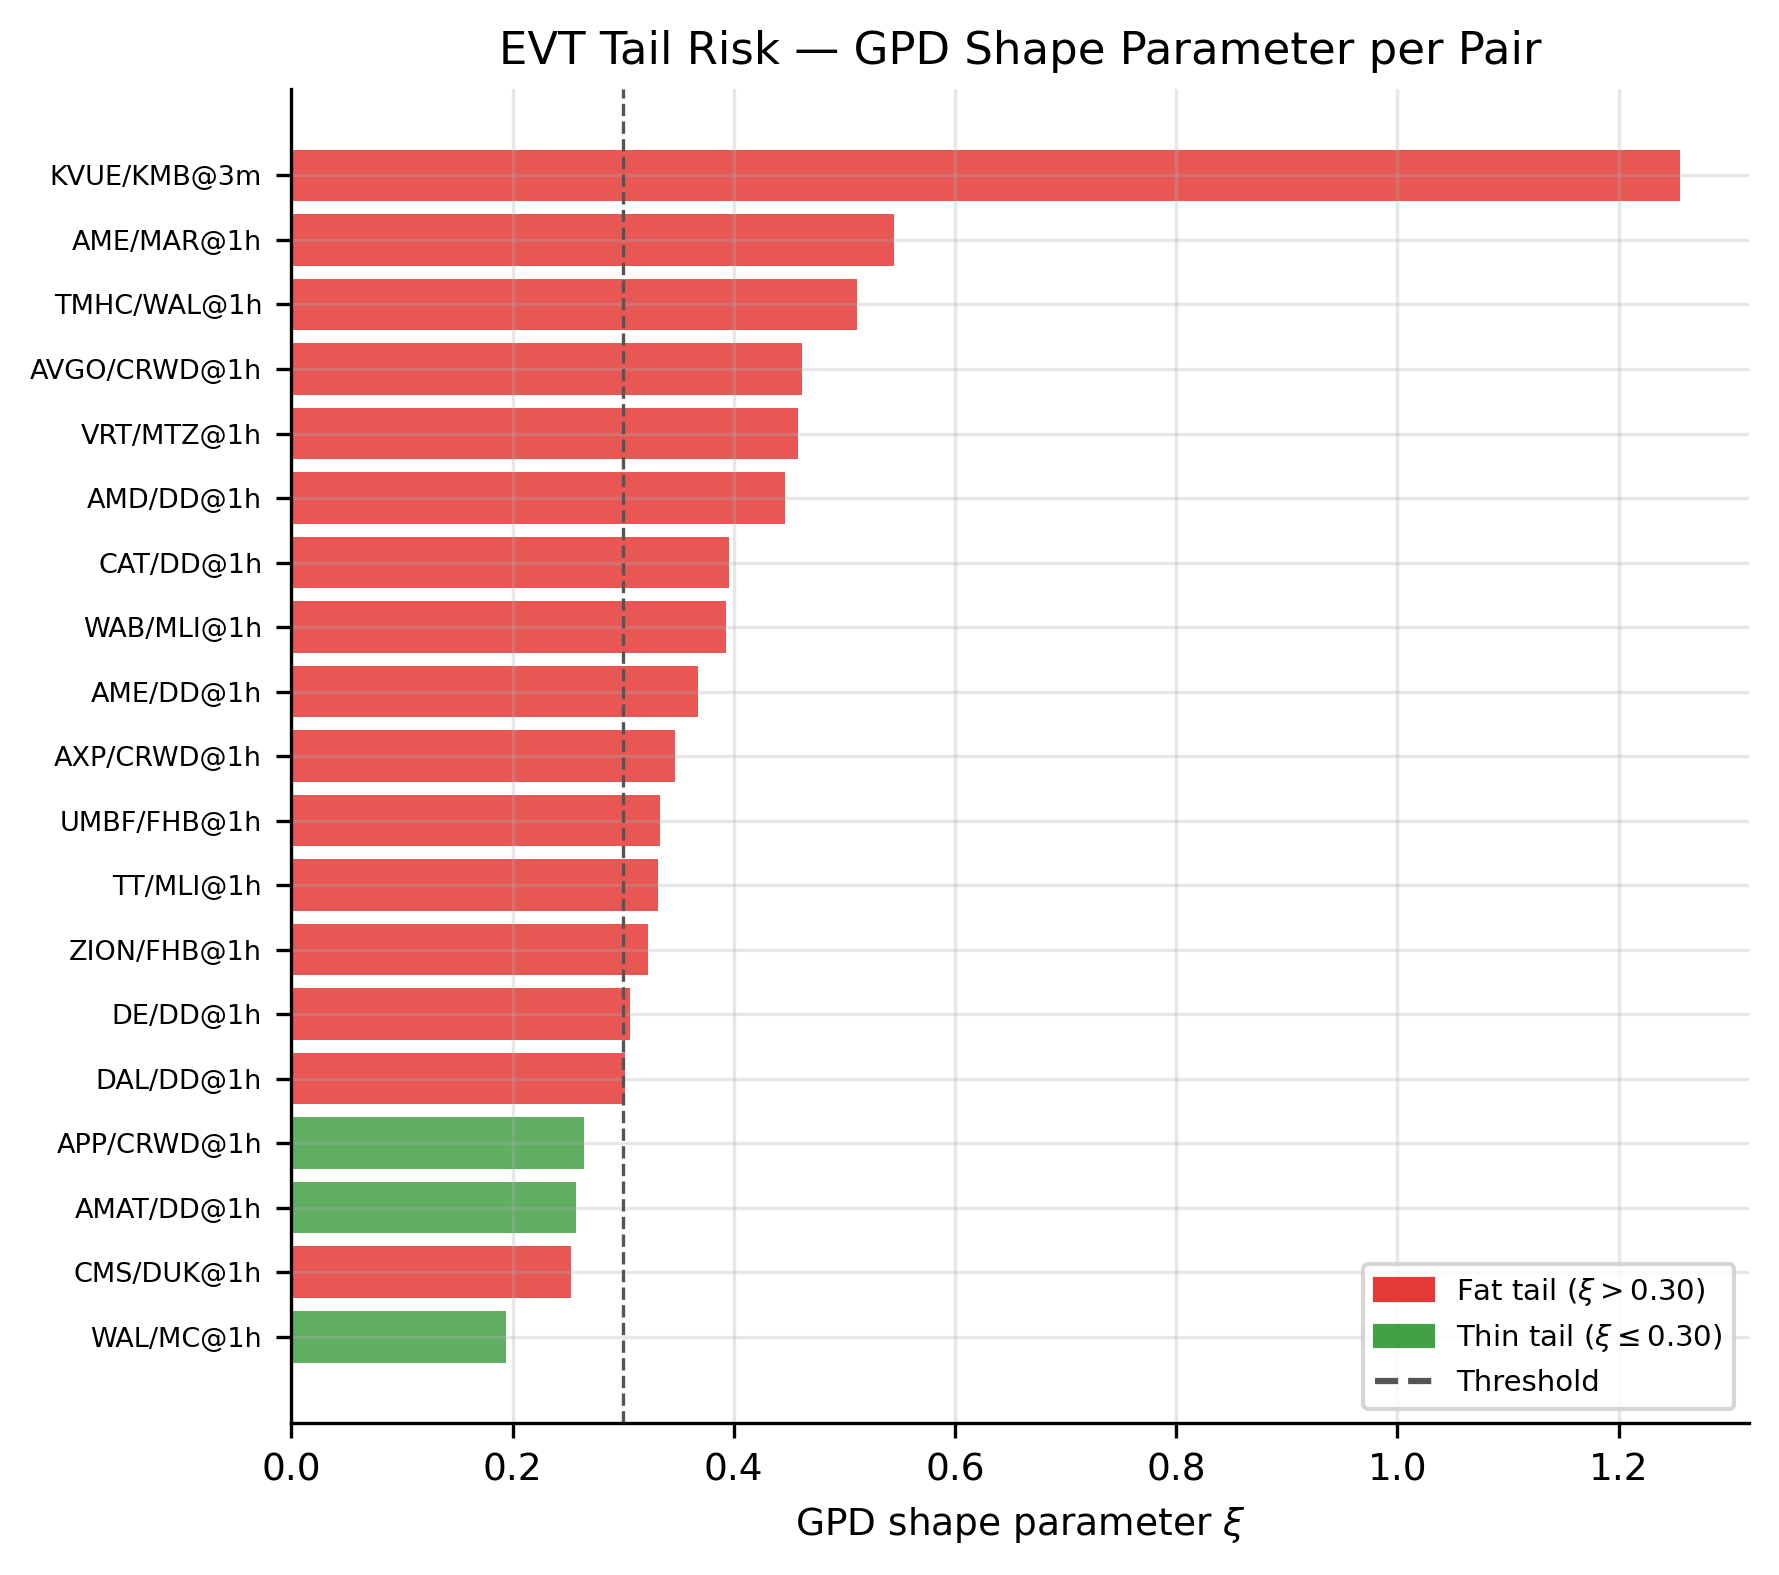
\includegraphics[width=0.80\textwidth]{figures/evt_tail_risk.png}
\caption{GPD shape parameter $\xi$ per pair. Red bars: fat-tailed ($\xi > 0.30$).}
\label{fig:evt}
\end{figure}

\begin{figure}[htbp]
\centering
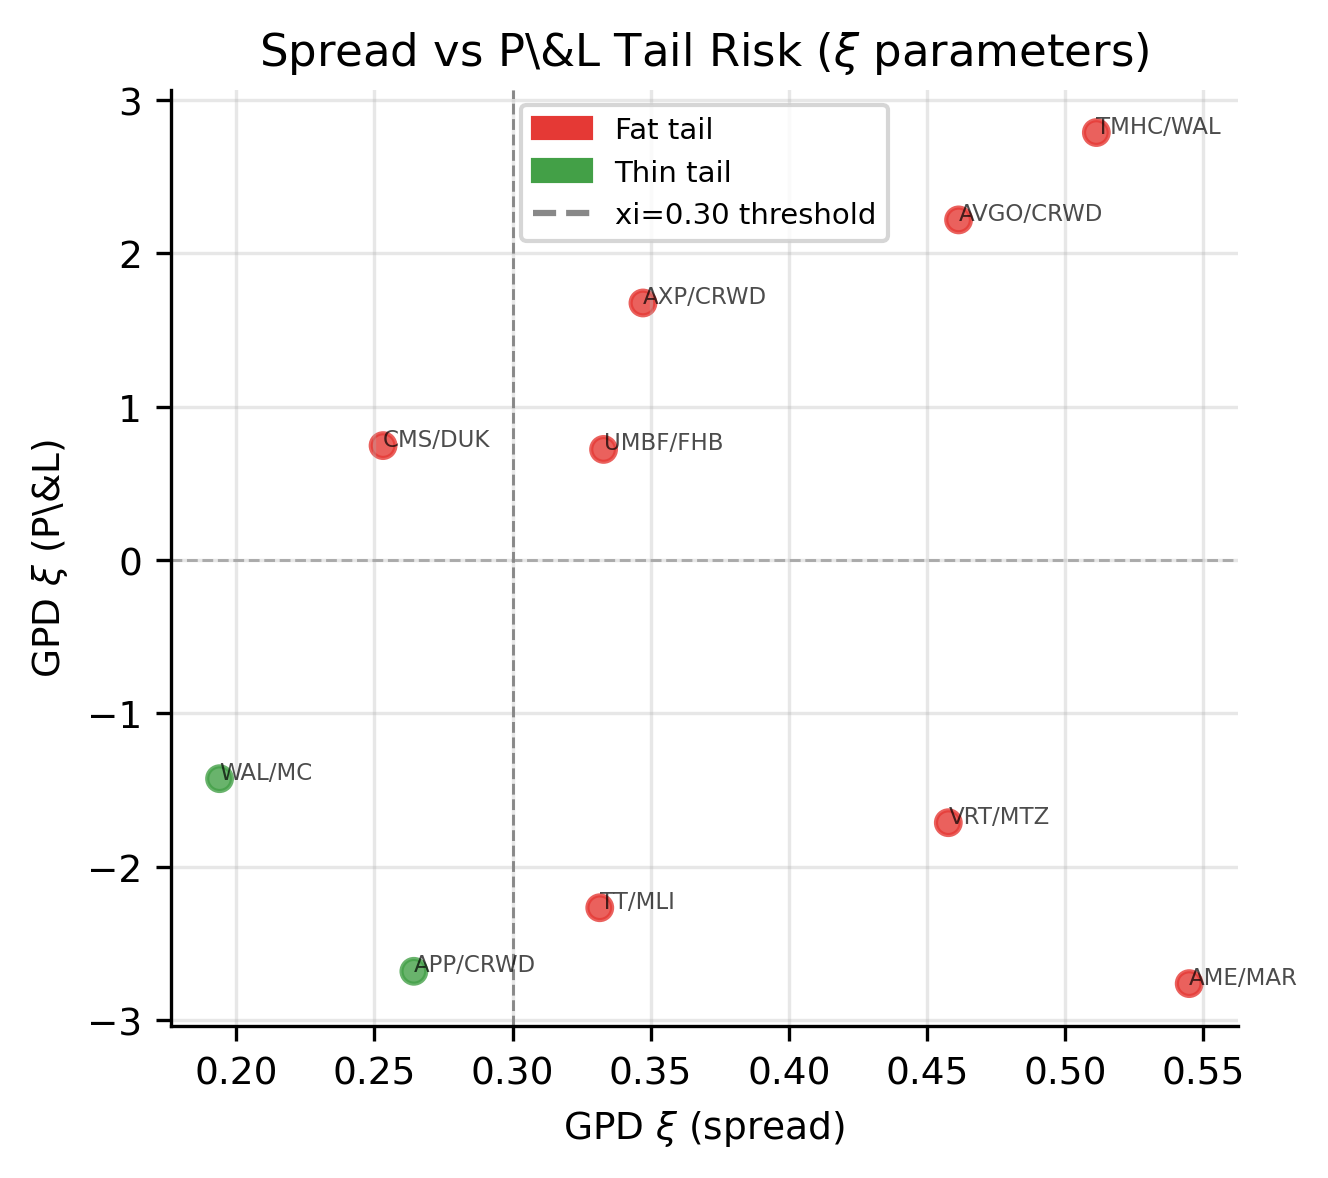
\includegraphics[width=0.60\textwidth]{figures/evt_xi_scatter.png}
\caption{Spread $\xi$ vs P\&L $\xi$. Fat-tailed spreads do not always produce fat-tailed P\&L.}
\label{fig:evt_xi_scatter}
\end{figure}

\begin{figure}[htbp]
\centering
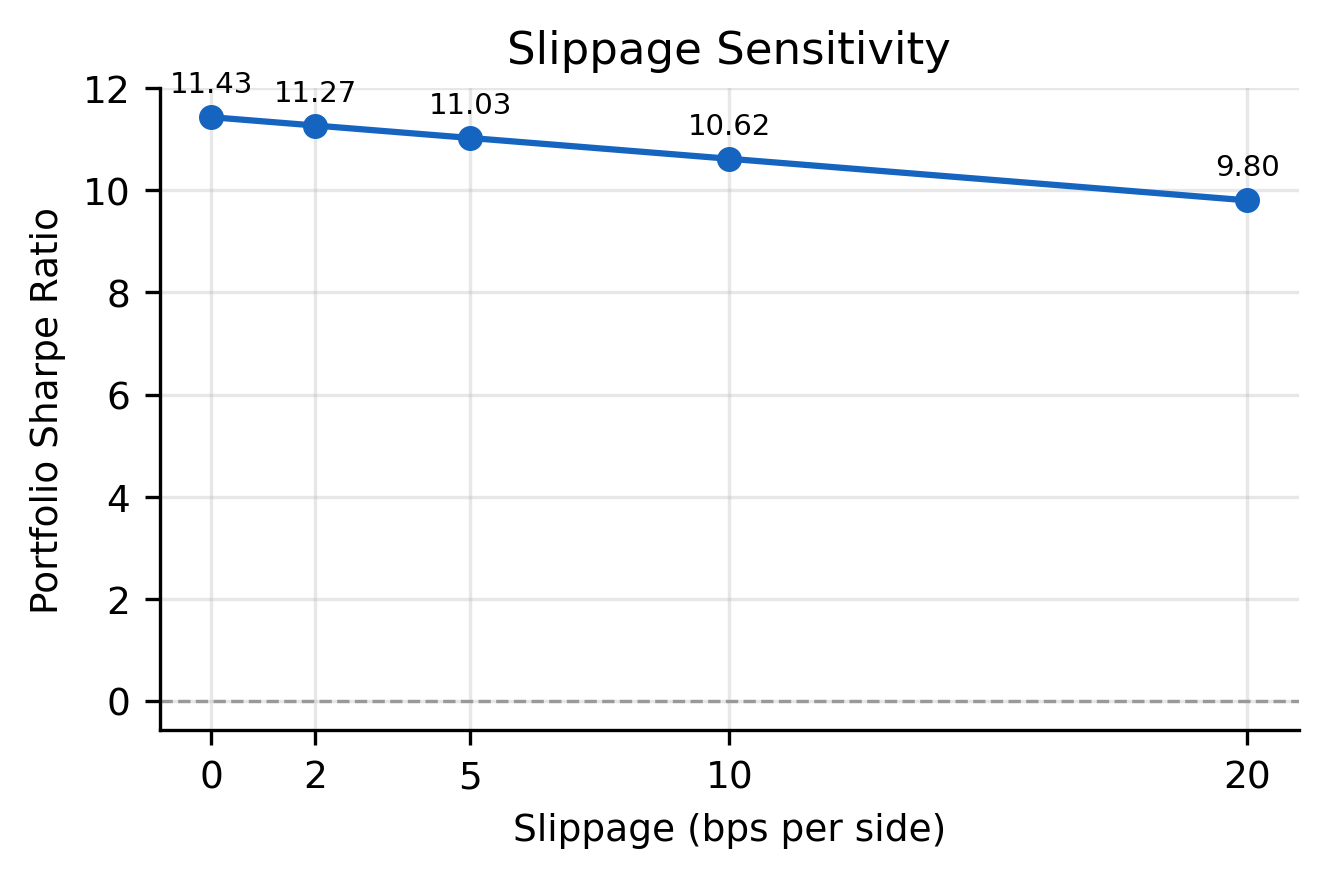
\includegraphics[width=0.65\textwidth]{figures/slippage_sensitivity.png}
\caption{Portfolio Sharpe as a function of per-side slippage.}
\label{fig:slippage}
\end{figure}

\begin{figure}[htbp]
\centering
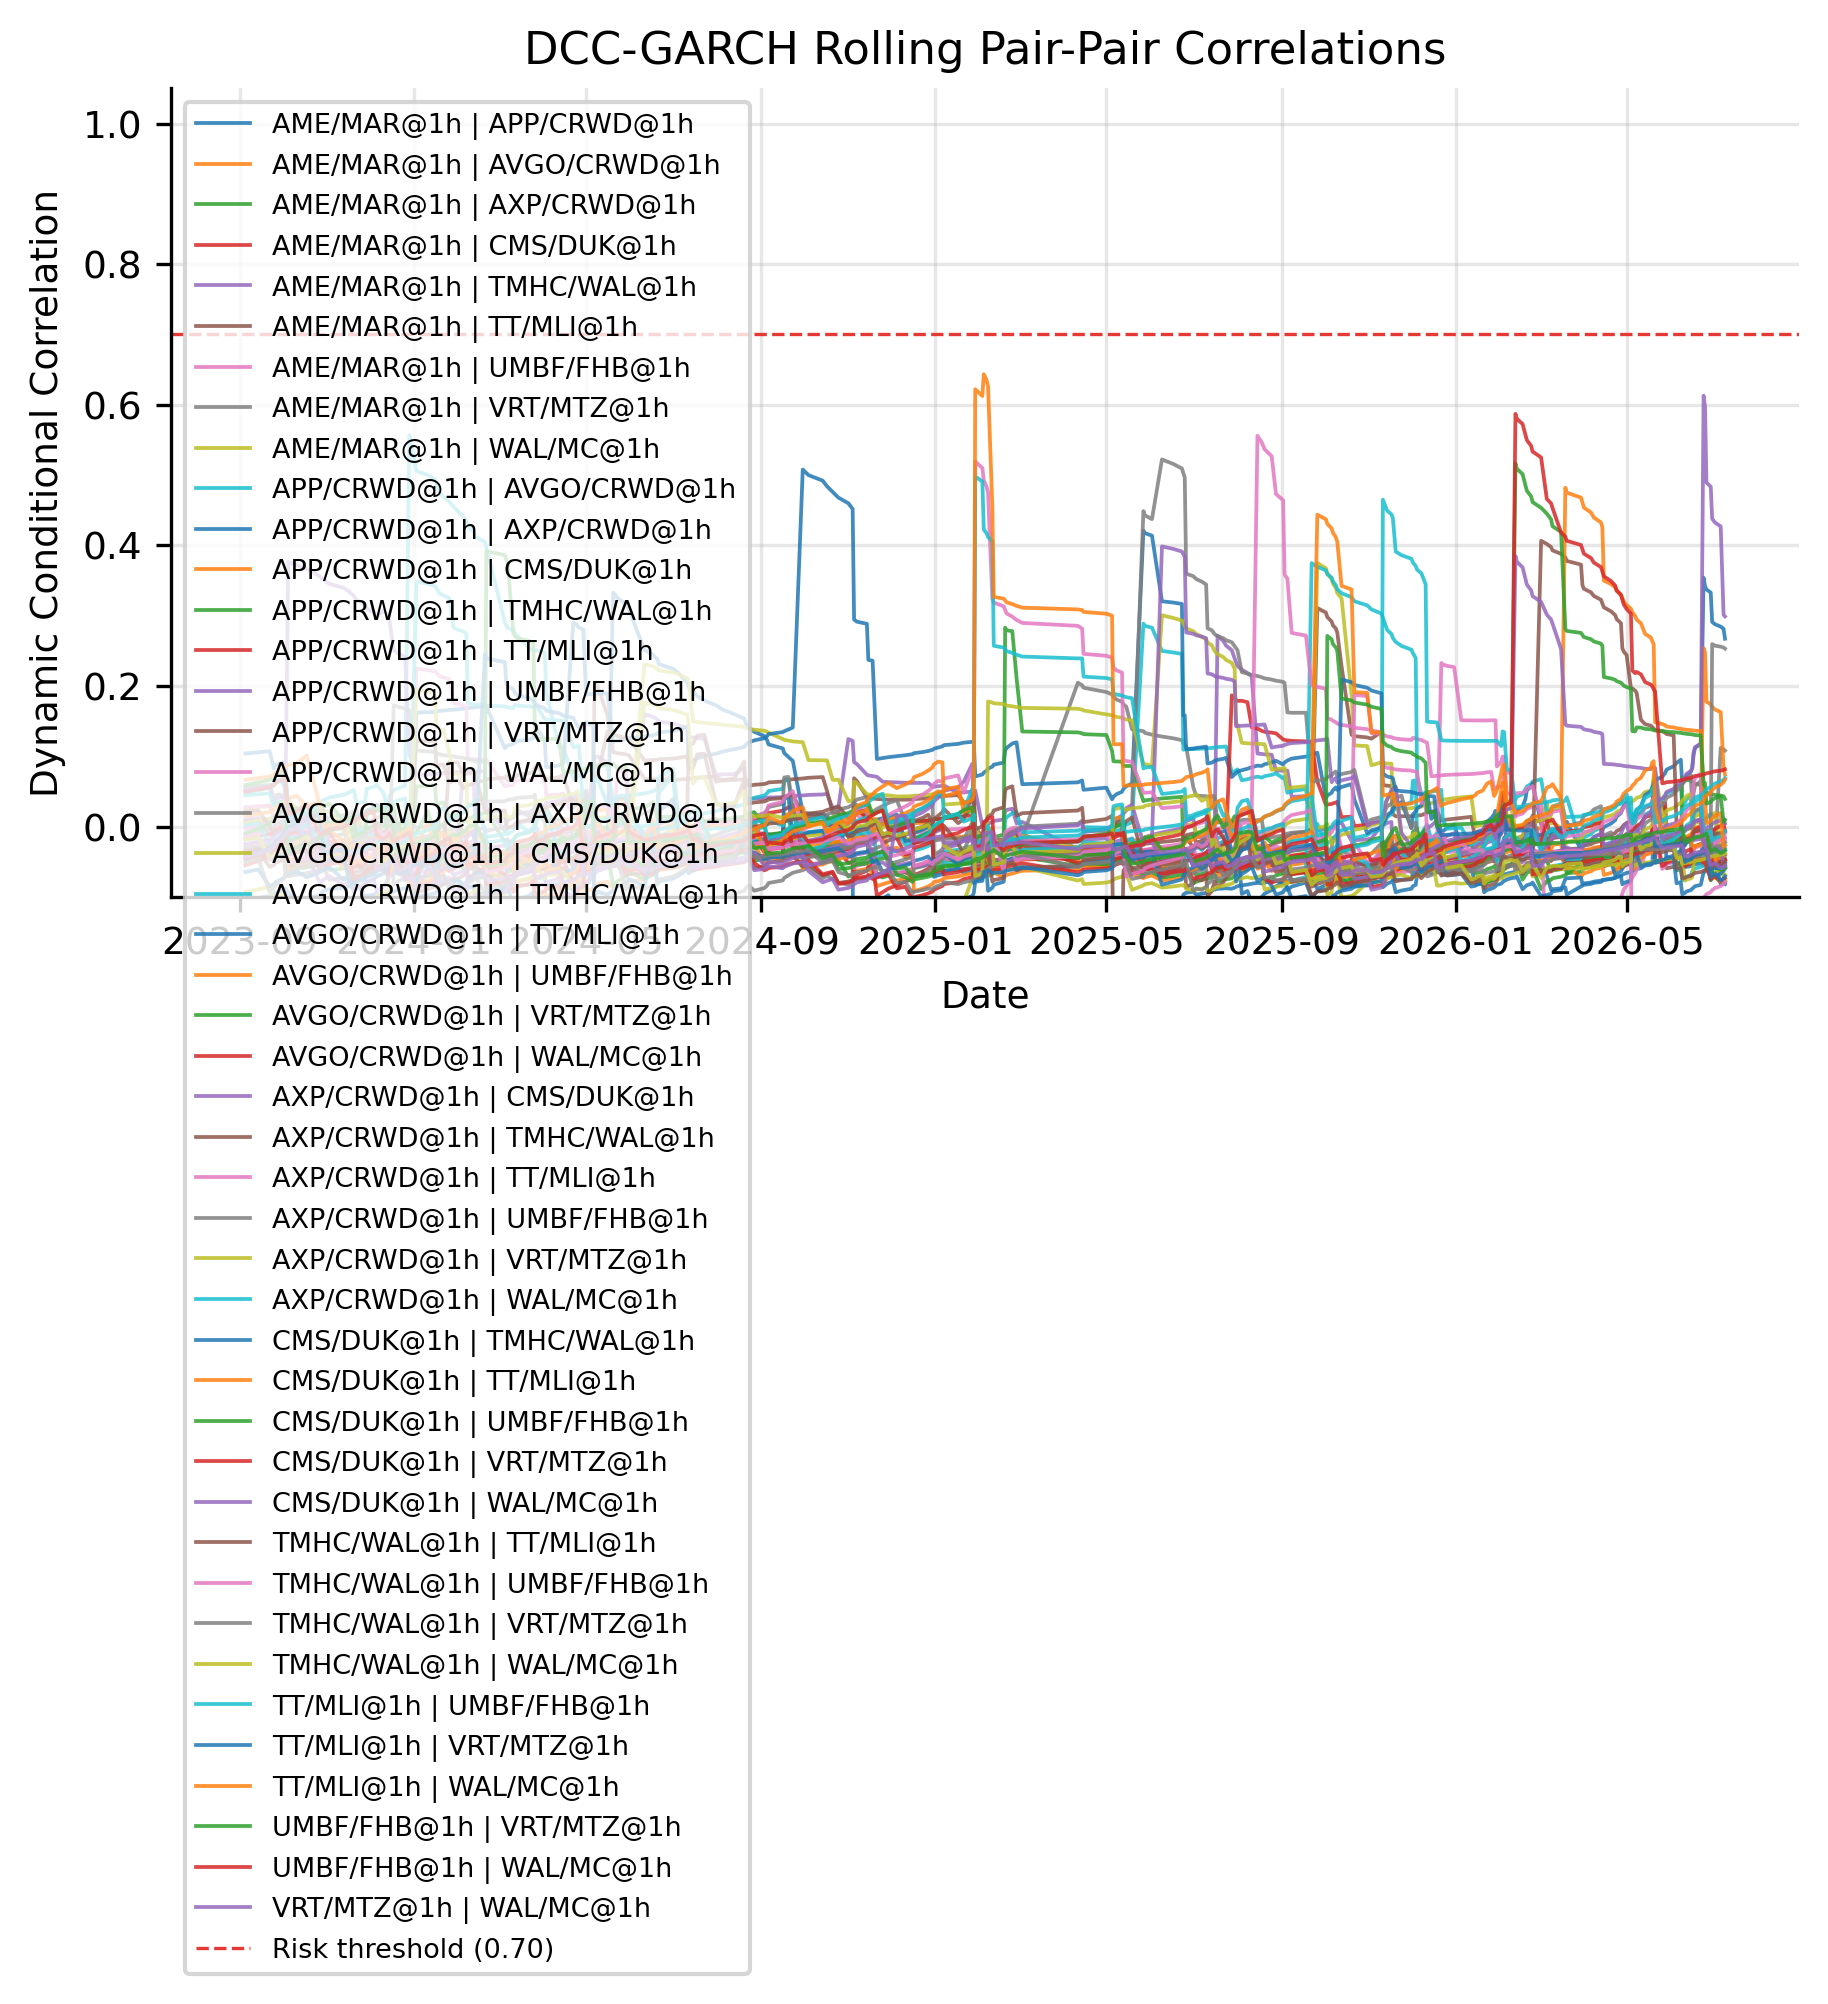
\includegraphics[width=0.90\textwidth]{figures/dcc_rolling.png}
\caption{DCC-GARCH rolling cross-pair correlations. Dashed line: 0.70 concentration-risk threshold.}
\label{fig:dcc}
\end{figure}

\begin{figure}[htbp]
\centering
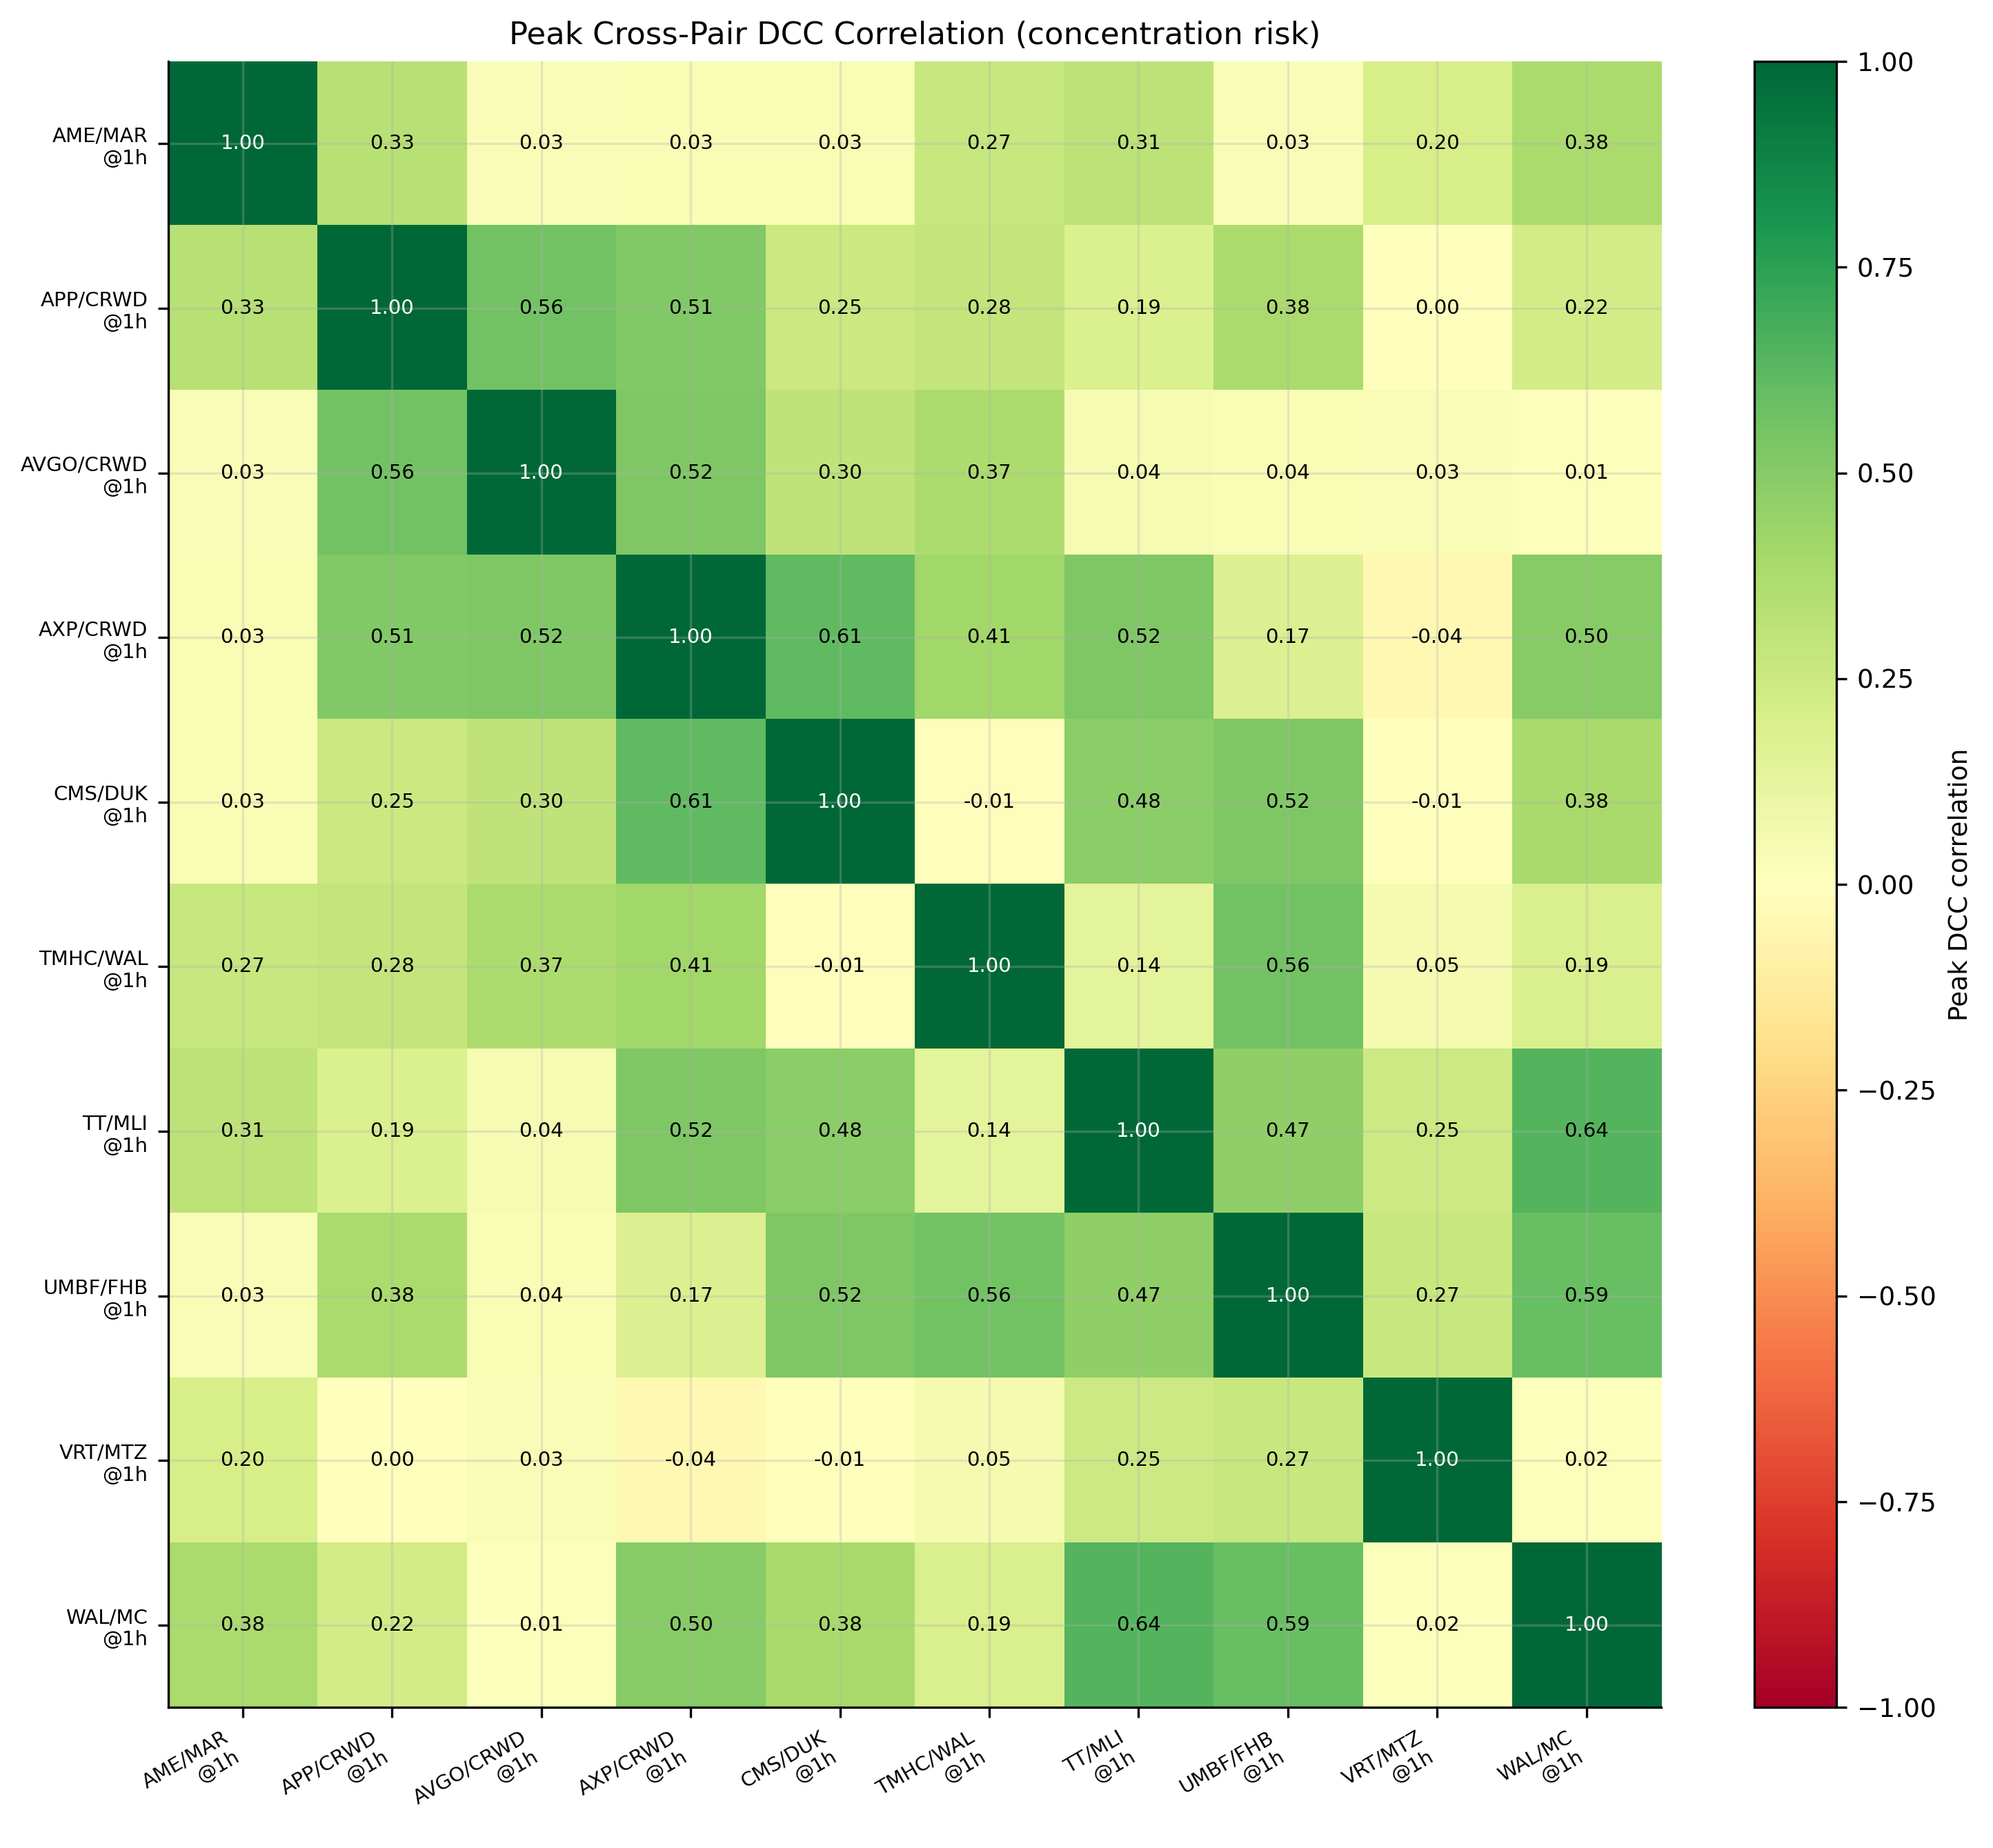
\includegraphics[width=0.70\textwidth]{figures/dcc_heatmap.png}
\caption{Peak pairwise DCC correlation heatmap. No pair-pair correlation exceeds 0.30.}
\label{fig:dcc_heatmap}
\end{figure}

\begin{figure}[htbp]
\centering
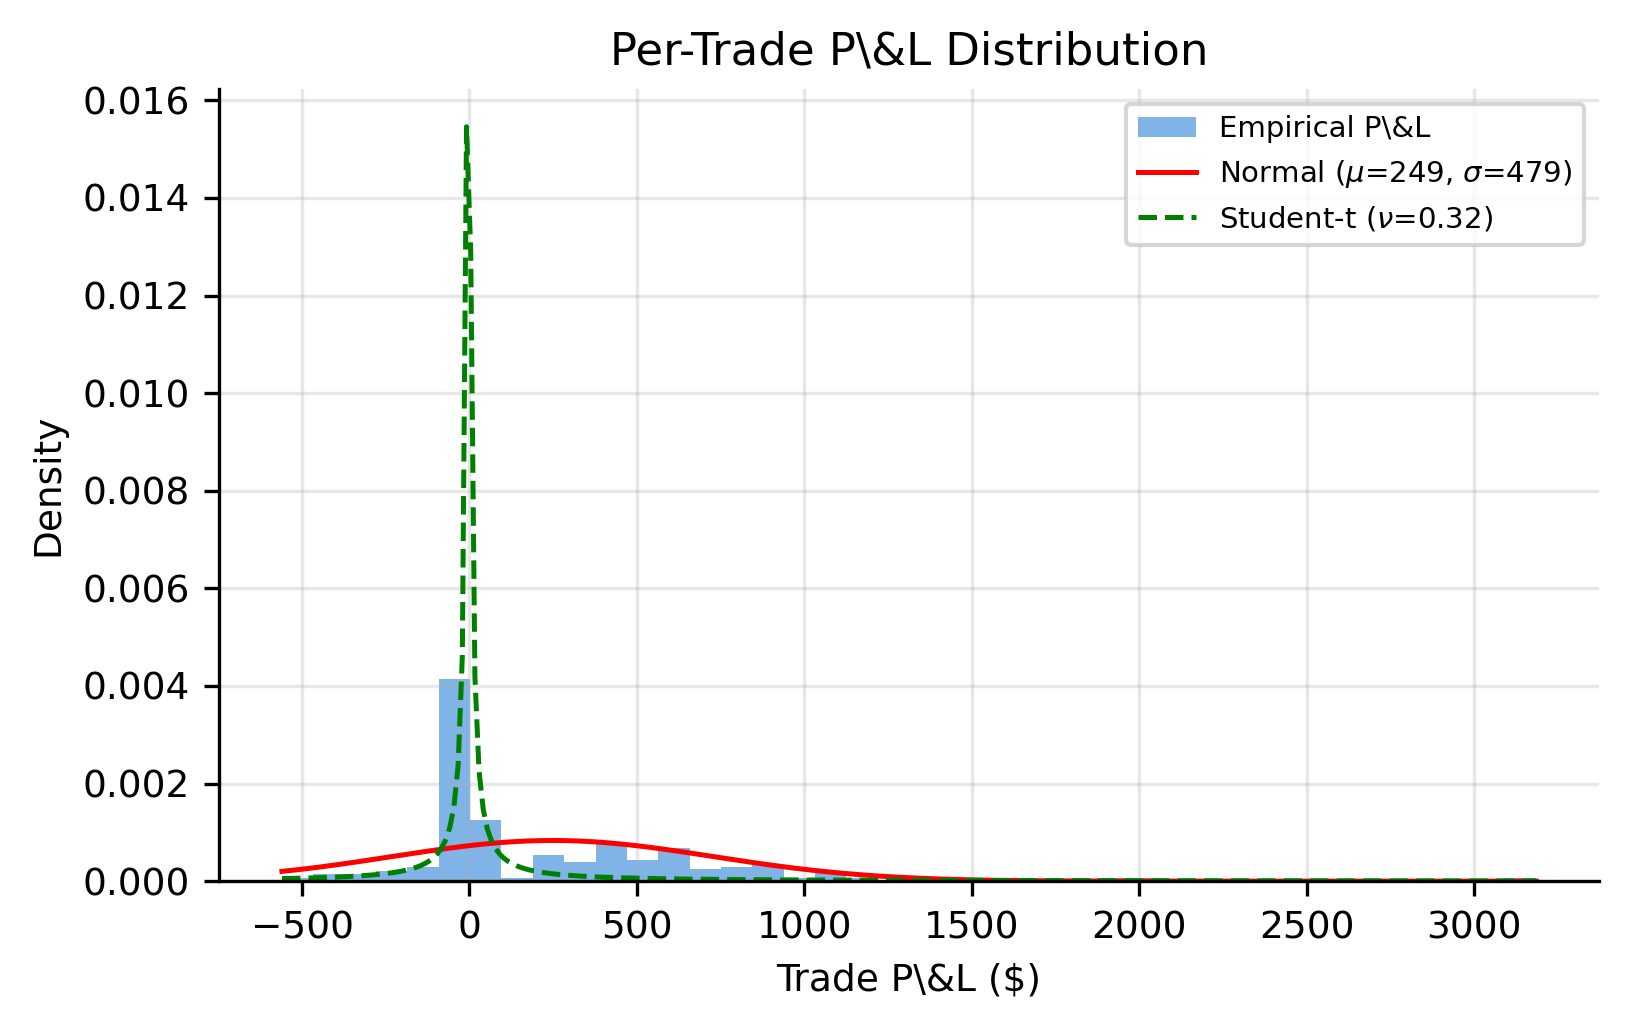
\includegraphics[width=0.75\textwidth]{figures/mc_distribution.png}
\caption{Per-trade P\&L distribution with Normal and Student-$t$ overlays.}
\label{fig:mc}
\end{figure}

\begin{figure}[htbp]
\centering
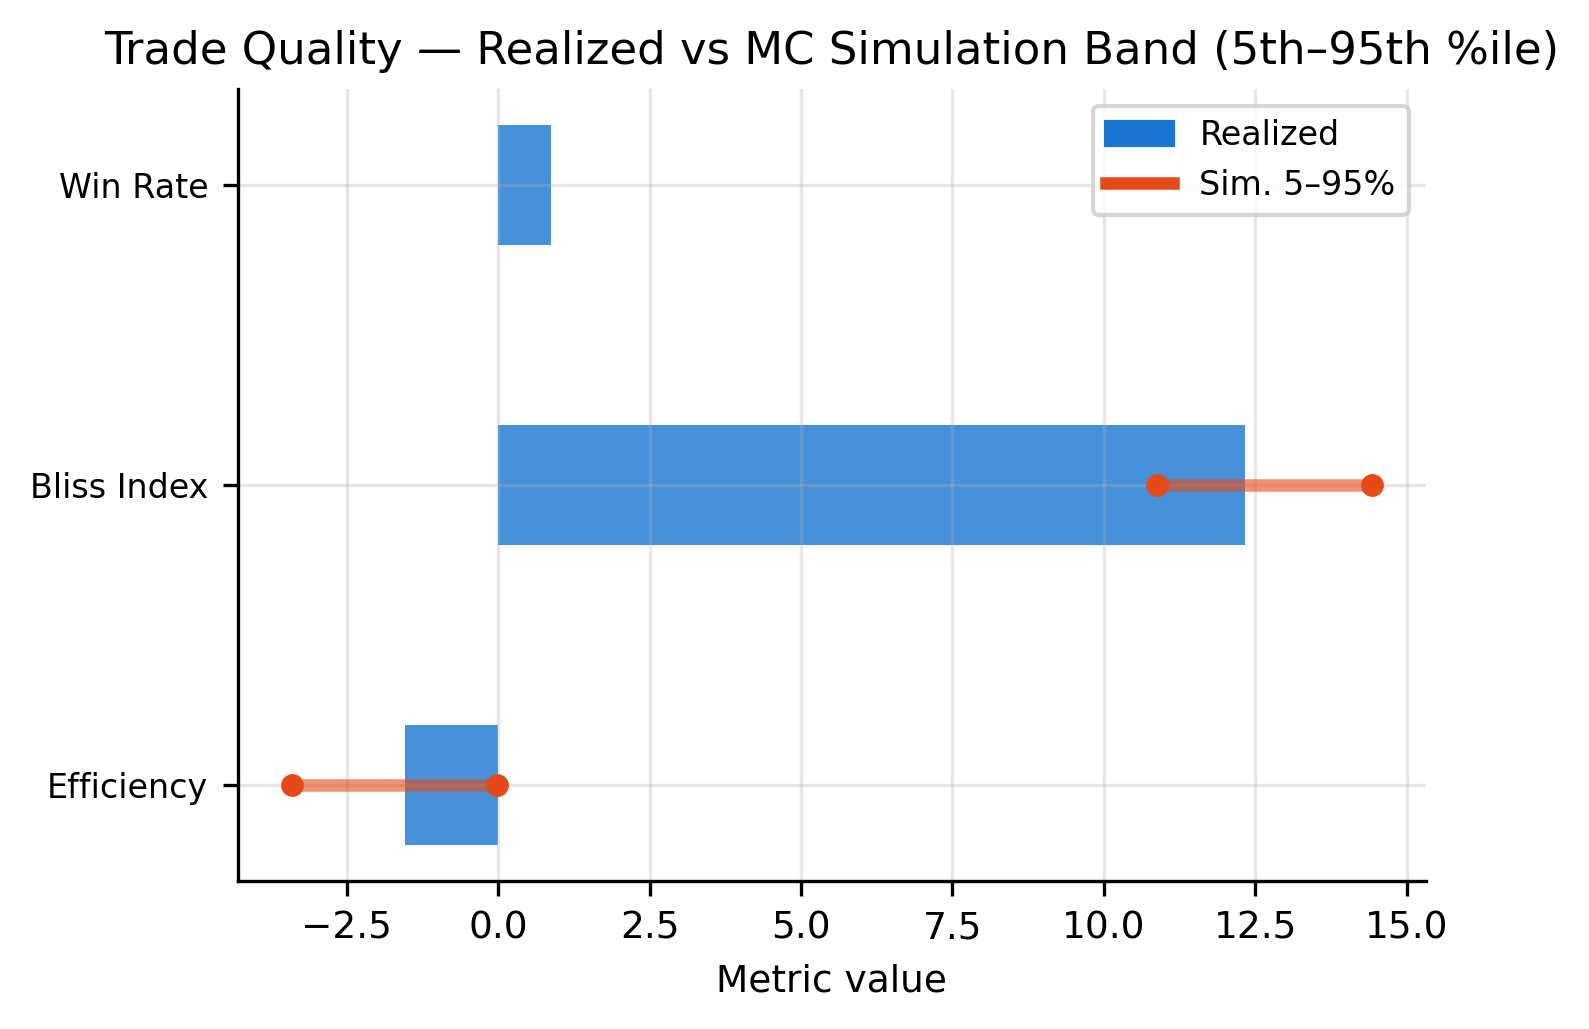
\includegraphics[width=0.65\textwidth]{figures/mc_quality.png}
\caption{Trade quality metrics (efficiency, bliss, win rate) vs MC simulation 5th--95th percentile band.}
\label{fig:mc_quality}
\end{figure}

\begin{figure}[htbp]
\centering
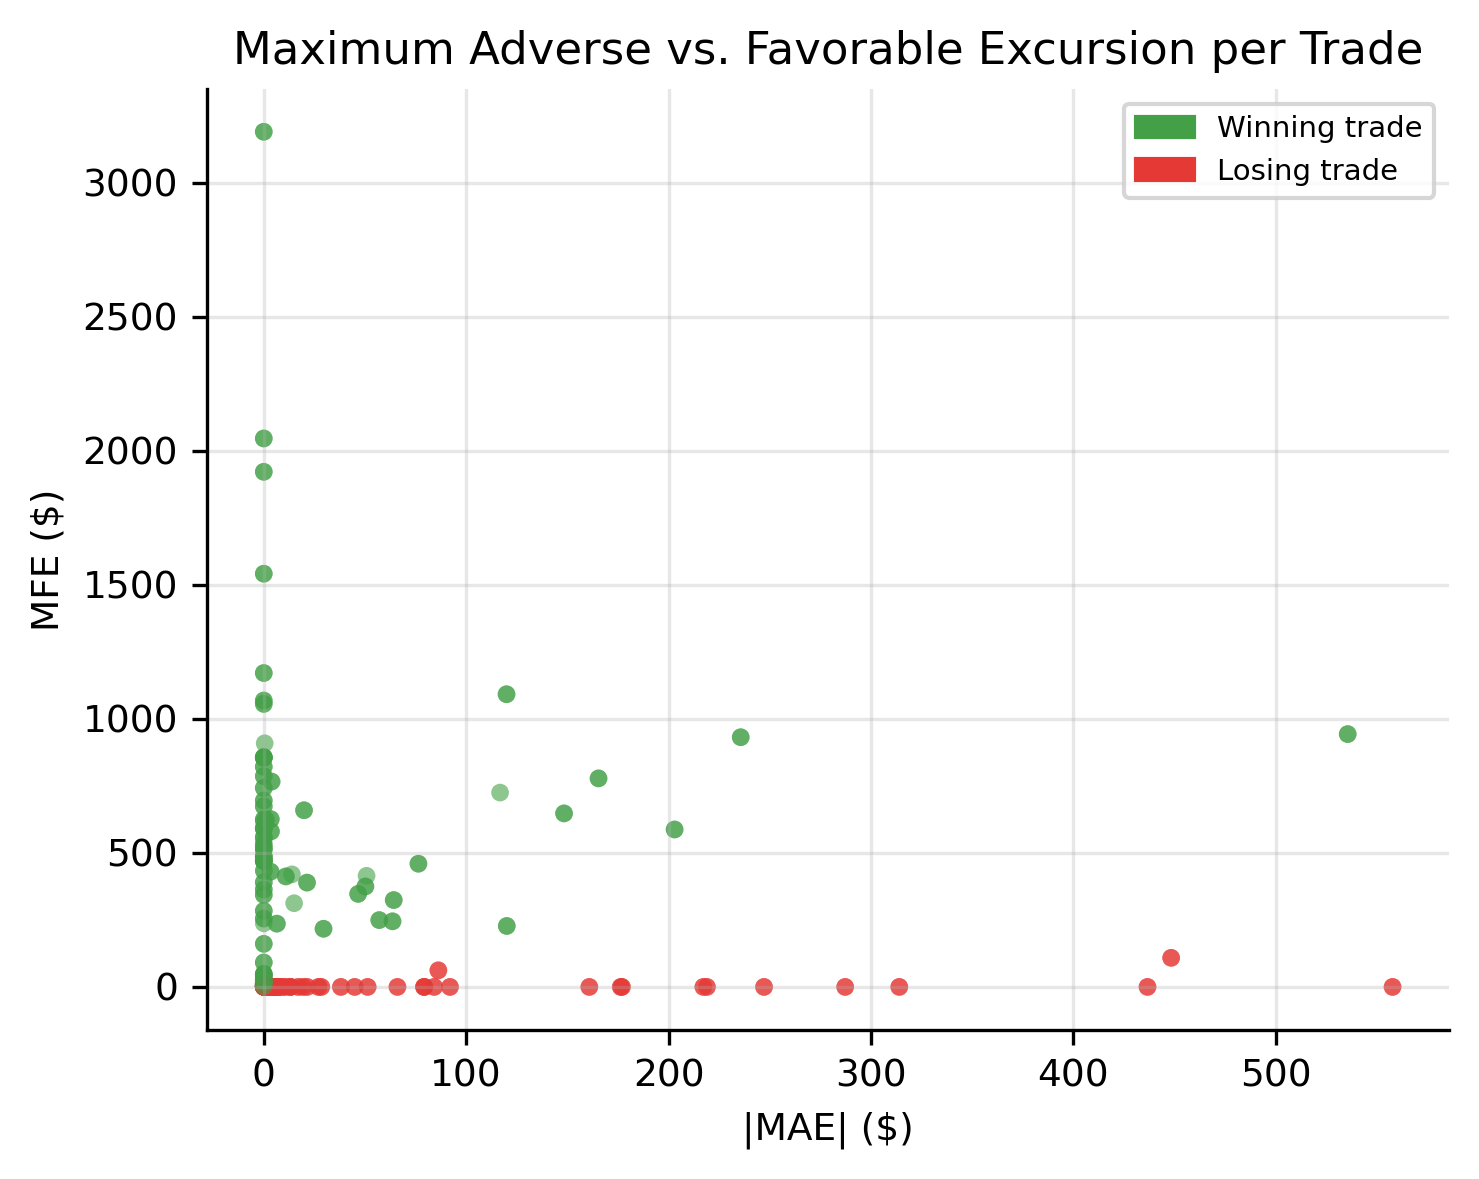
\includegraphics[width=0.65\textwidth]{figures/mfe_mae.png}
\caption{Maximum Adverse Excursion vs.\ Maximum Favorable Excursion per trade.}
\label{fig:mfe}
\end{figure}

\begin{figure}[htbp]
\centering
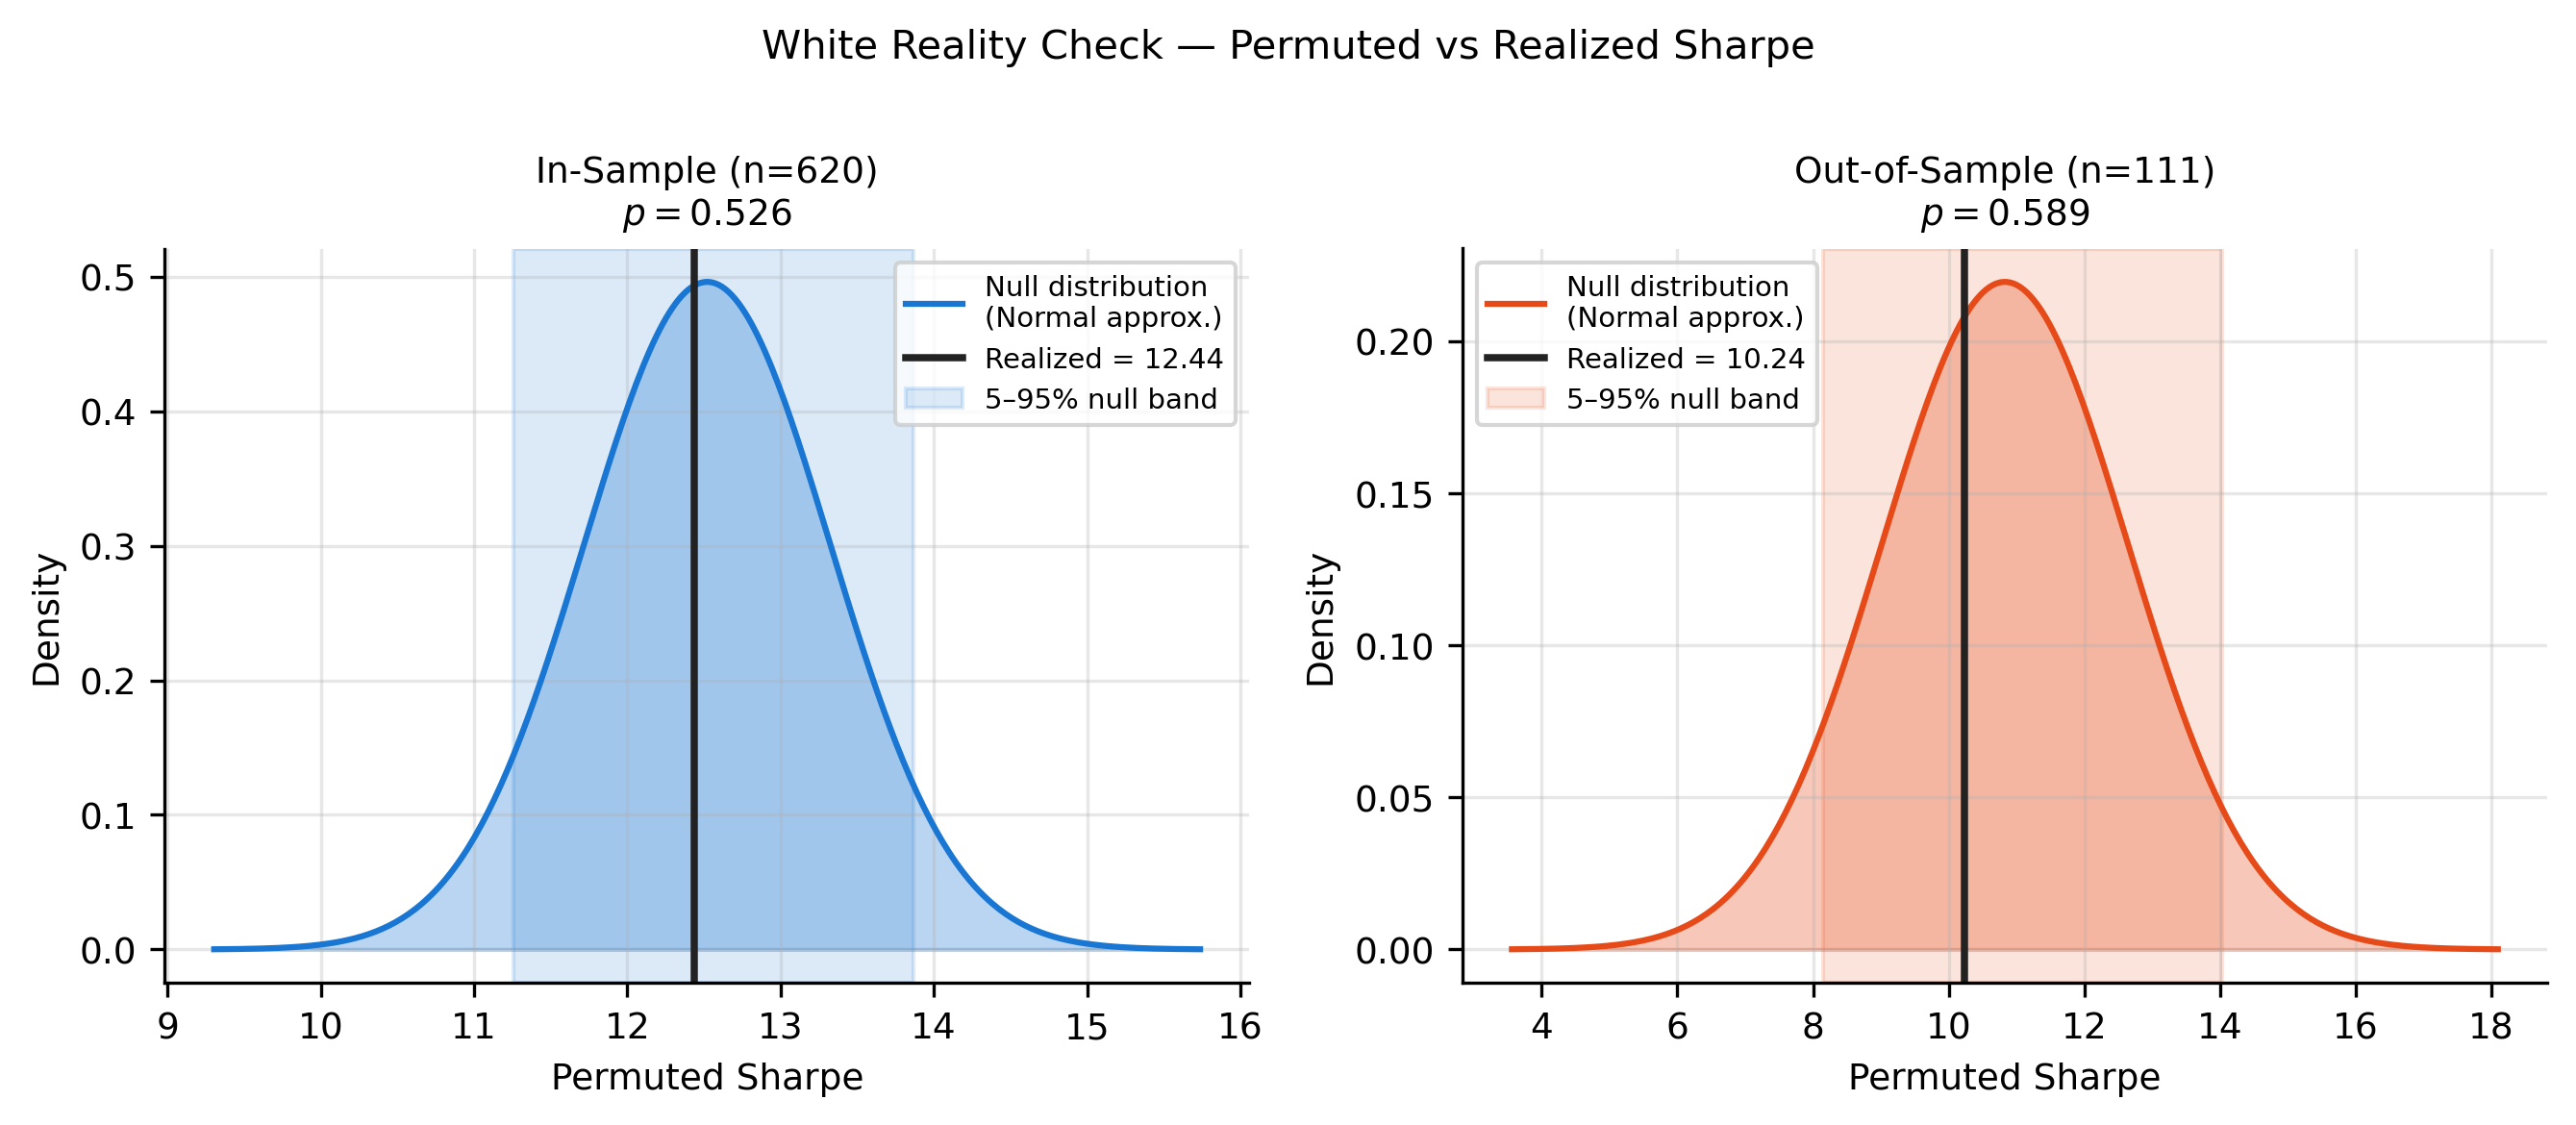
\includegraphics[width=0.90\textwidth]{figures/perm_distribution.png}
\caption{White Reality Check: permuted vs realized closed-trade Sharpe (Normal approximation of null distribution).}
\label{fig:perm_dist}
\end{figure}

\begin{figure}[htbp]
\centering
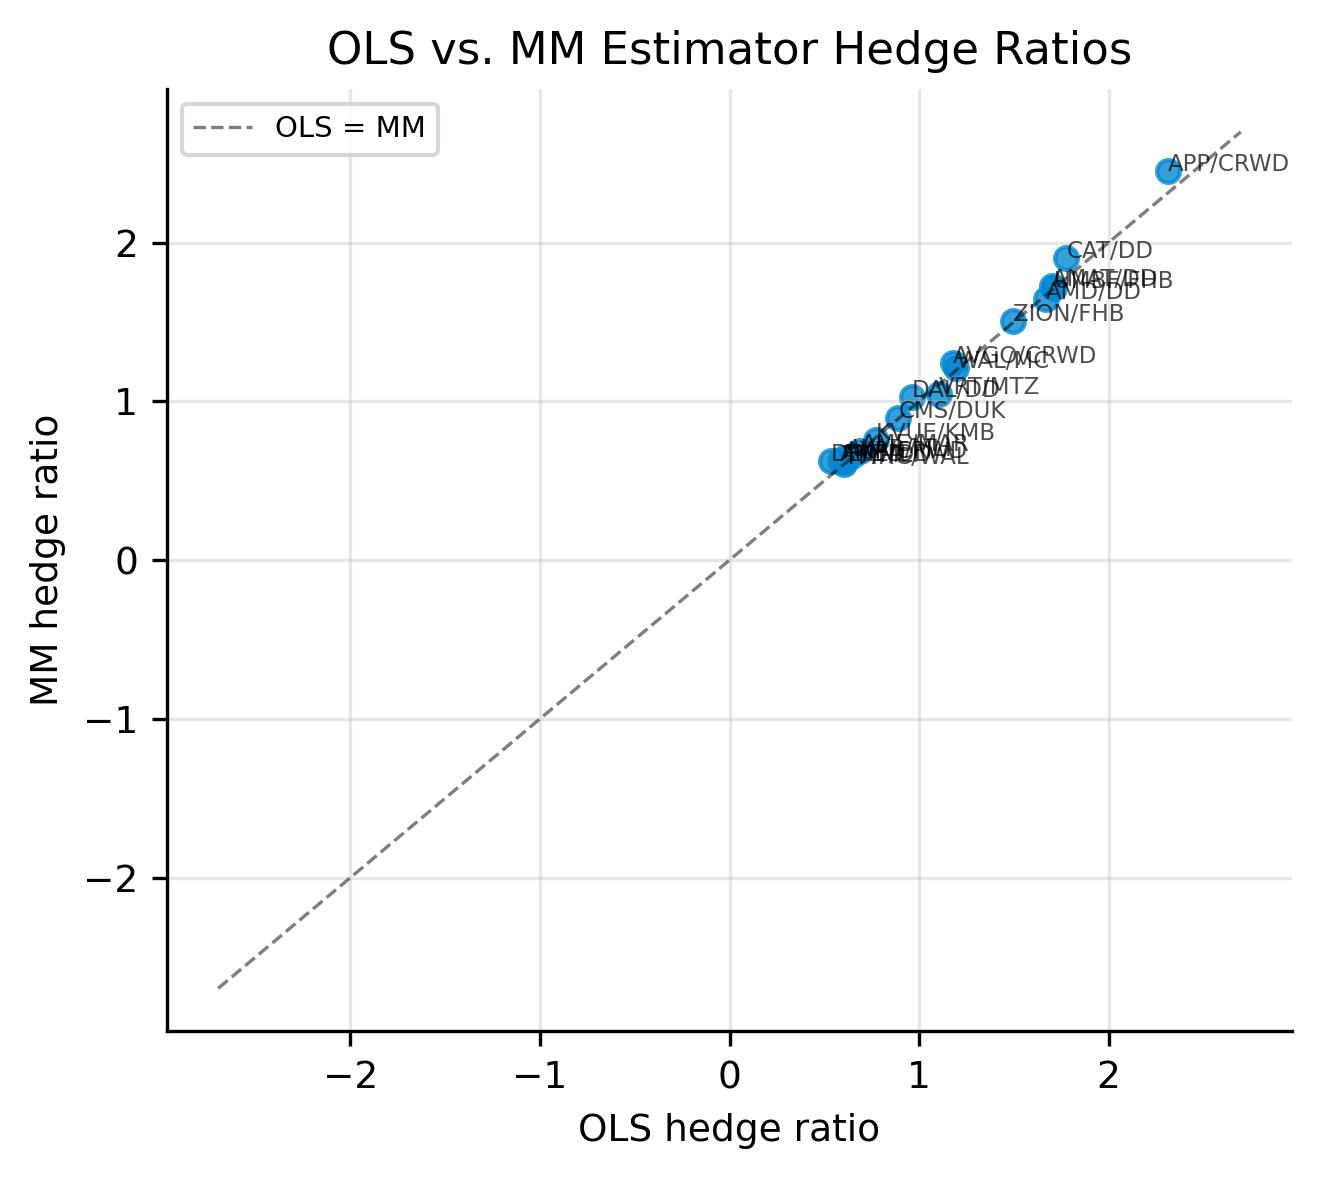
\includegraphics[width=0.65\textwidth]{figures/hedge_estimators.png}
\caption{OLS vs.\ MM hedge ratio estimates. Identity line in dashes.}
\label{fig:hedge}
\end{figure}

\begin{figure}[htbp]
\centering
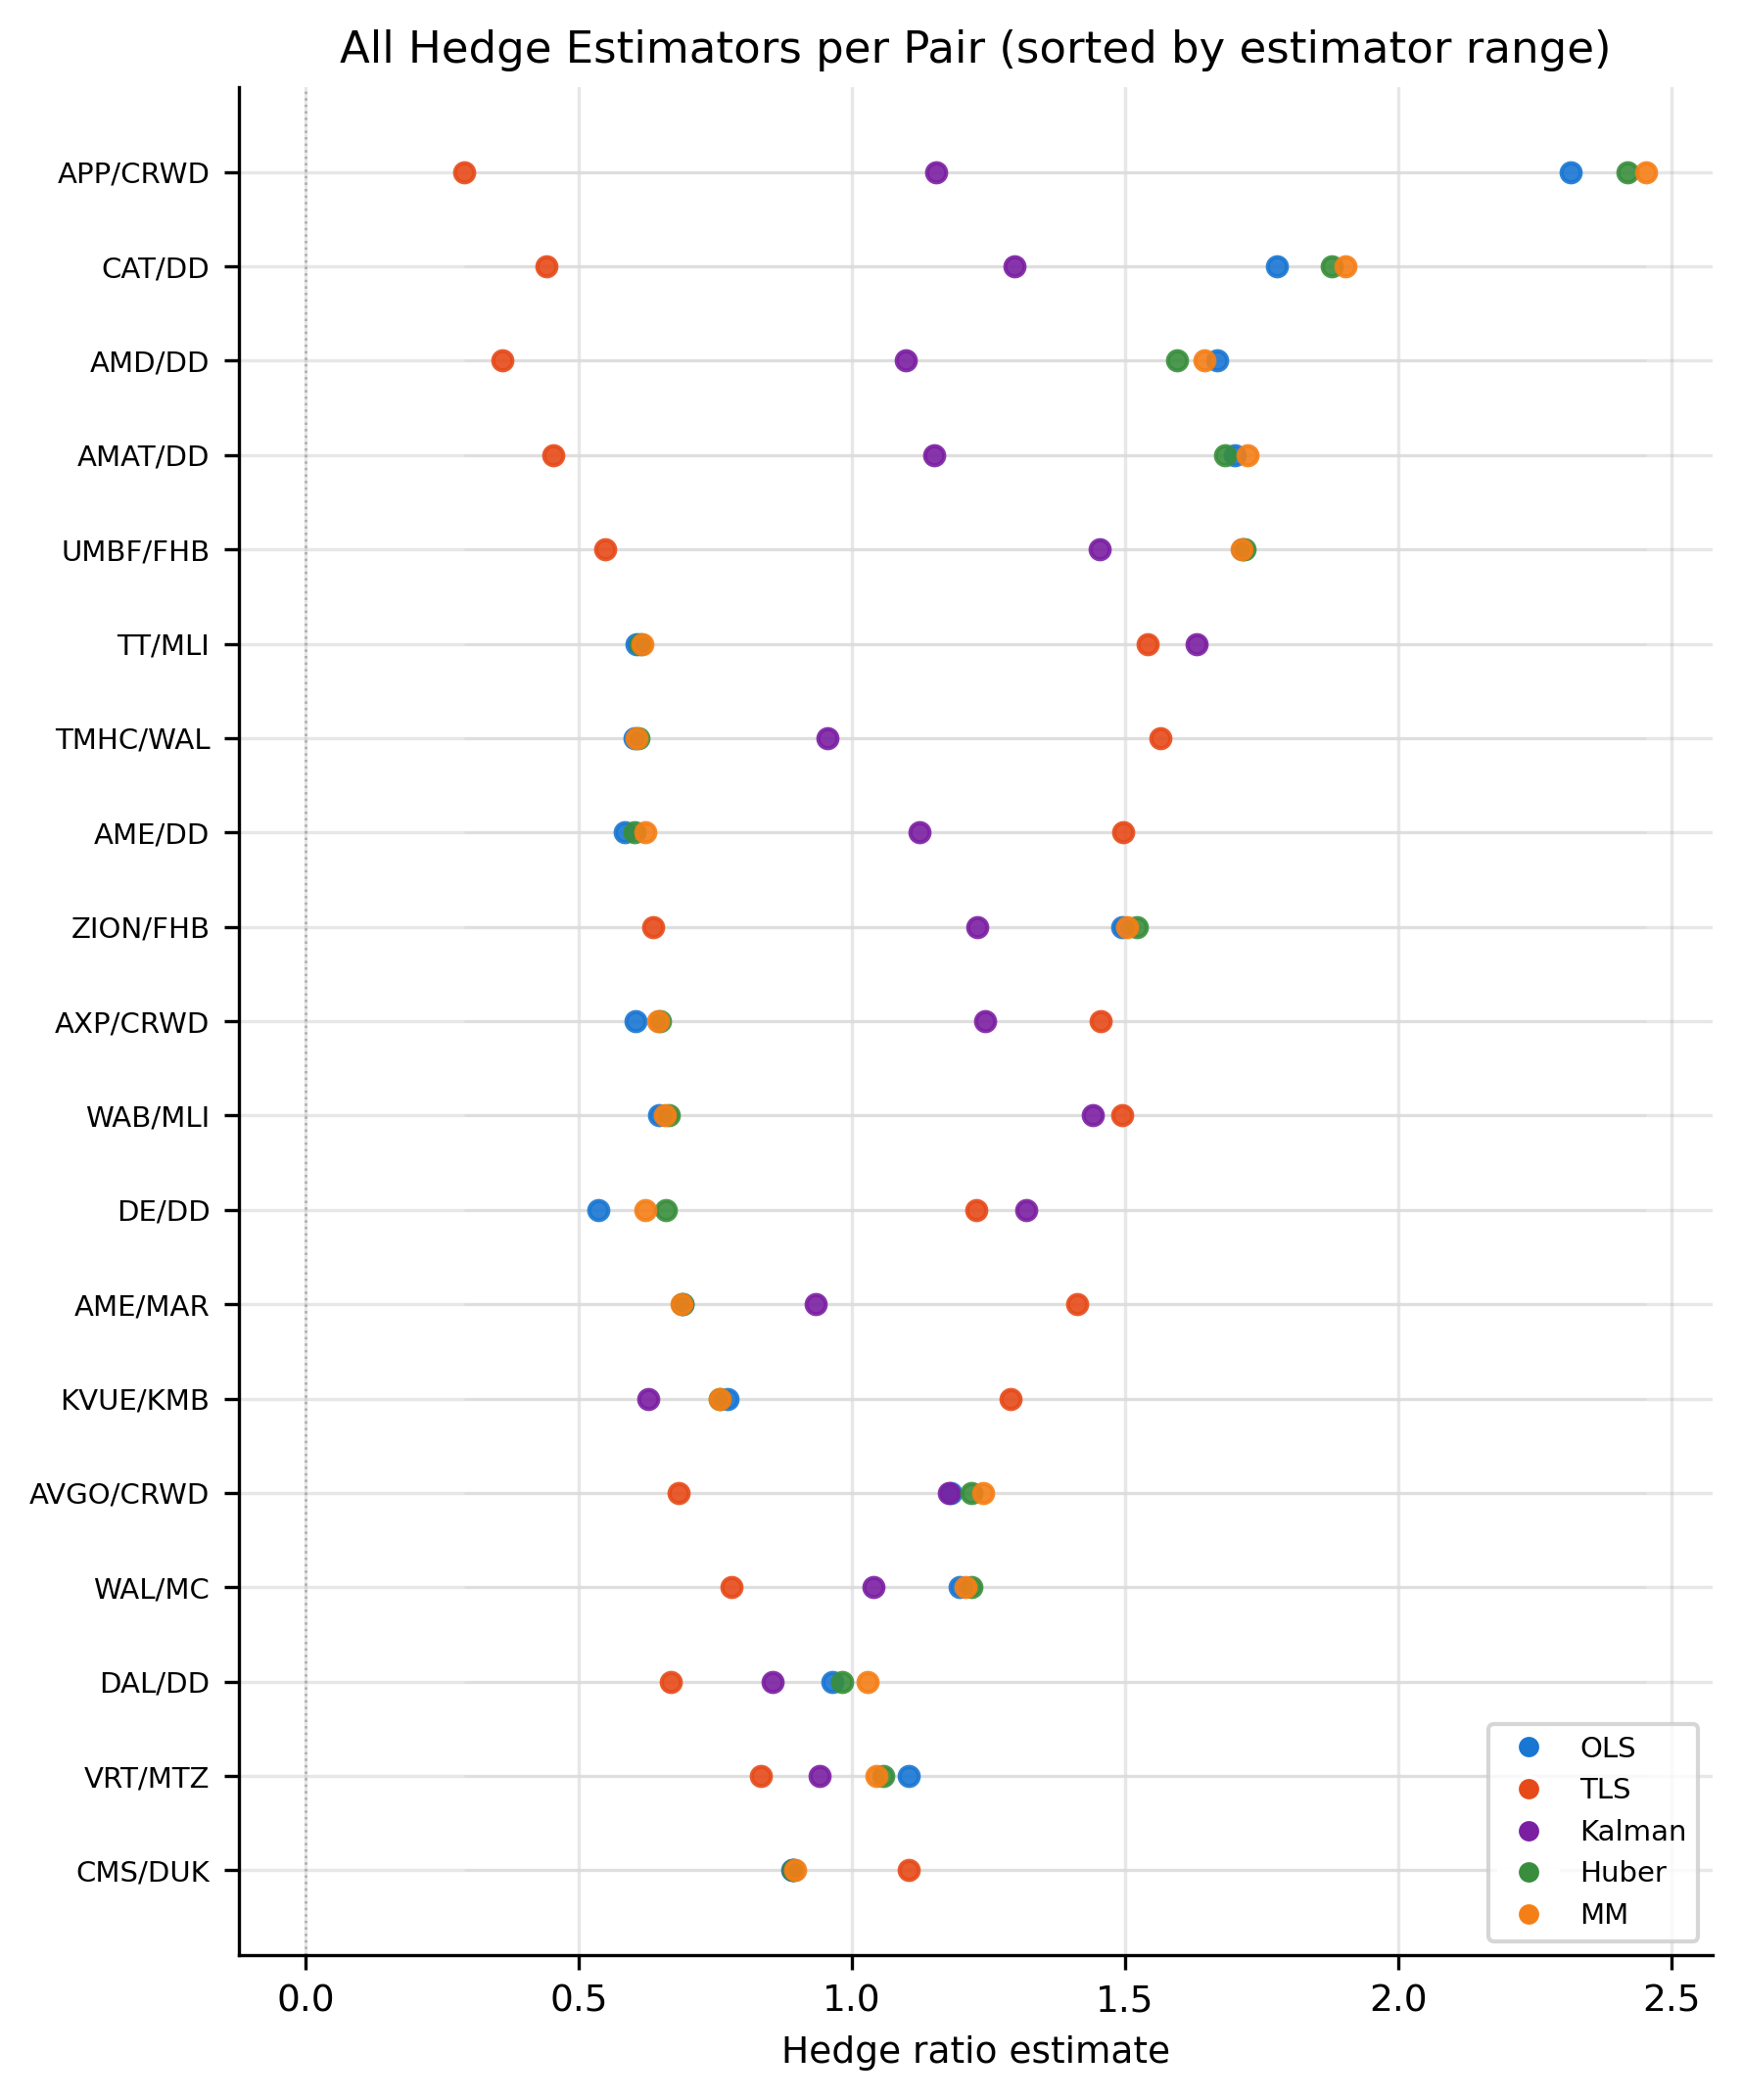
\includegraphics[width=0.80\textwidth]{figures/all_hedge_estimators.png}
\caption{All five hedge estimators per pair (Cleveland dot plot, sorted by estimator range).}
\label{fig:all_hedge_est}
\end{figure}


\section{Conclusion}

The central finding of this paper is methodological rather than strategic: the
full-sample Engle-Granger cointegration test, applied at daily and longer horizons,
exhibits a systematic failure mode---the Strictness Paradox---in which genuine
candidate pairs are rejected at rates orders of magnitude below the expected
false-positive rate. The cause is not an absence of cointegrated pairs; it is that
cointegration, when it exists at these horizons, is episodic rather than durable,
and the full-sample test cannot distinguish ``never cointegrated'' from ``cointegrated
in subperiods.''

The scalable rolling-stability diagnostic and three-test confirmatory tier system
introduced here address this directly. The resulting confirmed-pair set is smaller
but better calibrated. Out-of-sample strategy performance provides empirical evidence
that the calibration correction has teeth: the identified pairs generate positive
risk-adjusted returns that are not attributable to random timing (IS Reality Check
$p = 0.526$).

\subsection{Limitations}

\begin{itemize}
  \item ML meta-labeling layer is architecturally complete but awaiting sufficient
    training data ($n = 40$ labeled examples as of 2026-07-10; need 30/class).
  \item OOS permutation test power is limited (111 trades, 28 active days);
    the OOS result is deferred to future data accumulation.
  \item Universe restricted to U.S.\ equities + supplemental assets; international
    pairs not explored.
  \item No CRSP survivorship-bias correction; results may overstate universe
    coverage for pre-2000 periods.
\end{itemize}

\bibliographystyle{plainnat}
\bibliography{references}

\appendix

\section{Full Confirmed Pairs Table}
\begin{table}[htbp]
\centering
\footnotesize
\caption{Confirmed pairs with confirmatory cointegration tier. EG: Engle-Granger $p$-value (BH-FDR adjusted). Roll.\ Frac.: fraction of rolling windows confirming cointegration. KPSS: stationarity test $p$-value (want $>0.05$). PO: Phillips-Ouliaris proxy $p$-value (want $<0.10$). Significance: * $p<0.10$, ** $p<0.05$, *** $p<0.01$.}
\label{tab:confirmed_pairs}
\begin{tabular}{llcrrrrr}
\toprule
Pair & TF & Tier & EG $p$ & Roll. Frac. & KPSS $p$ & PO $p$ \\
\midrule
7267.T/8058.T & 1M & Bronze & 0.019 & 0.75 & --- & --- \\
AMD/DD & 1h & \textbf{Gold} & 0.013 & 0.04 & 0.208 & 0.000 \\
AME/DD & 1h & \textbf{Gold} & 0.000 & 0.07 & 0.402 & 0.000 \\
AMAT/DD & 1h & \textbf{Gold} & 0.000 & 0.04 & 0.236 & 0.000 \\
CMS/DUK & 1h & \textbf{Gold} & 0.016 & 0.06 & 0.065 & 0.000 \\
DAL/DD & 1h & \textbf{Gold} & 0.001 & 0.03 & 0.194 & 0.000 \\
TT/MLI & 1h & \textbf{Gold} & 0.000 & 0.07 & 0.467 & 0.000 \\
TMHC/WAL & 1h & \textbf{Gold} & 0.040 & 0.14 & 0.090 & 0.000 \\
UMBF/FHB & 1h & \textbf{Gold} & 0.039 & 0.18 & 0.439 & 0.000 \\
AXP/CRWD & 1h & Silver & 0.021 & 0.01 & 0.000 & 0.000 \\
AME/MAR & 1h & Silver & 0.011 & 0.09 & 0.005 & 0.000 \\
APP/CRWD & 1h & Silver & 0.044 & 0.09 & 0.006 & 0.000 \\
AVGO/CRWD & 1h & Silver & 0.005 & 0.06 & 0.000 & 0.000 \\
CAT/DD & 1h & Silver & 0.000 & 0.07 & 0.004 & 0.000 \\
DE/DD & 1h & Silver & 0.049 & 0.11 & 0.000 & 0.000 \\
VRT/MTZ & 1h & Silver & 0.002 & 0.08 & 0.000 & 0.000 \\
WAB/MLI & 1h & Silver & 0.000 & 0.11 & 0.013 & 0.000 \\
WAL/MC & 1h & Silver & 0.044 & 0.06 & 0.000 & 0.000 \\
ZION/FHB & 1h & Silver & 0.030 & 0.16 & 0.002 & 0.000 \\
KVUE/KMB & 3m & Silver & 0.001 & 0.99 & 0.000 & 0.000 \\
\bottomrule
\end{tabular}
\end{table}

\section{Backtest Variant Performance}
\begin{table}[htbp]
\centering
\small
\caption{Portfolio-level performance across all backtest variants. IS = in-sample (full history). OOS = out-of-sample (20\% chronological holdout). Sharpe annualized assuming 252 trading days. Max DD = maximum peak-to-trough drawdown in dollars.}
\label{tab:perf_variants}
\begin{tabular}{lrrrrrrr}
\toprule
Variant & Trades & Sharpe & Calmar & Total P\&L & Max DD & Win Rate & Pairs \\
\midrule
IS (Layer 1) & 1042 & 5.40 & --- & \$302,114 & \$3,702 & 0.67 & 12 \\
OOS Baseline & 296 & 5.24 & --- & \$73,596 & \$1,227 & 0.61 & 15 \\
OOS Huber-weighted & 296 & 5.02 & --- & \$51,857 & \$963 & 0.61 & 15 \\
OOS + Neg-hedge & 304 & 5.45 & --- & \$77,740 & \$1,229 & 0.64 & 15 \\
OOS P\&L-cap & 296 & 5.24 & --- & \$73,596 & \$1,227 & 0.61 & 15 \\
OOS Risk-parity & 296 & 5.87 & --- & \$62,490 & \$1,136 & 0.61 & 15 \\
\bottomrule
\end{tabular}
\end{table}

\section{EVT Tail Risk Table}
\begin{table}[htbp]
\centering
\small
\caption{GPD extreme value theory fit per pair. $\xi > 0$ indicates a fat-tailed (Pareto) distribution; $\xi > 0.30$ triggers the fat-tail flag. Threshold: 95th percentile of absolute spread changes.}
\label{tab:evt_risk}
\begin{tabular}{llrrrrc}
\toprule
Pair & TF & $\xi$ (spread) & $\sigma$ (spread) & $\xi$ (P\&L) & Fat tail? \\
\midrule
KVUE/KMB & 3m & 1.255 & 0.1 & --- & \checkmark \\
AME/MAR & 1h & 0.545 & 0.0 & -2.762 & \checkmark \\
TMHC/WAL & 1h & 0.511 & 0.1 & 2.788 & \checkmark \\
AVGO/CRWD & 1h & 0.461 & 0.1 & 2.219 & \checkmark \\
VRT/MTZ & 1h & 0.458 & 0.1 & -1.713 & \checkmark \\
AMD/DD & 1h & 0.446 & 0.2 & --- & \checkmark \\
CAT/DD & 1h & 0.396 & 0.1 & --- & \checkmark \\
WAB/MLI & 1h & 0.393 & 0.0 & --- & \checkmark \\
AME/DD & 1h & 0.368 & 0.1 & --- & \checkmark \\
AXP/CRWD & 1h & 0.347 & 0.0 & 1.677 & \checkmark \\
UMBF/FHB & 1h & 0.333 & 0.0 & 0.722 & \checkmark \\
TT/MLI & 1h & 0.332 & 0.0 & -2.267 & \checkmark \\
ZION/FHB & 1h & 0.323 & 0.0 & --- & \checkmark \\
DE/DD & 1h & 0.307 & 0.1 & --- & \checkmark \\
DAL/DD & 1h & 0.302 & 0.1 & --- & \checkmark \\
APP/CRWD & 1h & 0.264 & 0.1 & -2.682 & --- \\
AMAT/DD & 1h & 0.258 & 0.2 & --- & --- \\
CMS/DUK & 1h & 0.253 & 0.0 & 0.747 & \checkmark \\
WAL/MC & 1h & 0.194 & 0.1 & -1.426 & --- \\
7267.T/8058.T & 1M & --- & --- & --- & --- \\
\bottomrule
\end{tabular}
\end{table}

\section{Permutation Test Results}
\begin{table}[htbp]
\centering
\small
\caption{White (2000) Reality Check permutation test. Null: entry signal timing has no skill --- \texttt{pnl\_net} values randomly reassigned across trades, exit-date structure preserved. $p$-value = fraction of $N=1{,}000$ permuted closed-trade Sharpes $\geq$ realized. OOS result has limited power (111 trades, 28 active days).}
\label{tab:permutation}
\begin{tabular}{lrrrrrrl}
\toprule
Sample & N trades & N days & Realized Sharpe & Perm. mean & Perm. 95\%ile & $p$-value & Significant? \\
\midrule
In-sample & 1042 & 284 & 12.44 & 12.52 & 13.87 & 0.526 & No \\
Out-of-sample & 296 & 70 & 10.24 & 10.83 & 14.03 & 0.589 & No \\
\bottomrule
\end{tabular}
\end{table}

\section{Distribution Fitting}
\begin{table}[htbp]
\centering
\small
\caption{Best-fit distribution (minimum AIC) in bold. $k$ = number of parameters. $\dagger$: GARCH(1,1) fit on daily P\&L; AIC computed on standardized residuals.}
\label{tab:dist_fit}
\begin{tabular}{lrrrr}
\toprule
Distribution & $k$ & Log-lik. & AIC & BIC \\
\midrule
\textbf{GARCH(1,1) + Normal$^{\dagger}$} & 4 & -442.4 & \textbf{892.7} & 907.7 \\
Skew-Normal (NIG proxy) & 3 & -10085.1 & 20176.3 & 20191.9 \\
Laplace & 2 & -10090.8 & 20185.6 & 20196.0 \\
Student-$t$ & 3 & -10114.3 & 20234.6 & 20250.2 \\
Normal & 2 & -10173.8 & 20351.6 & 20362.0 \\
\bottomrule
\end{tabular}
\end{table}

\end{document}
